\documentclass[twoside, openright]{report}

\usepackage{tfg}

\makeglossaries

\begin{document}
	
	% PORTADA E INFORMACIÓN INICIAL
	\thispagestyle{empty}
\BgThispage

\begin{tikzpicture}[remember picture, overlay]
  \node[yshift=-5cm] at (current page.north west)
  {
    \begin{tikzpicture}[remember picture, overlay]
      \draw[fill = headingPortadaTFG, headingPortadaTFG, fill opacity = 1] (0,0) rectangle (\paperwidth,5cm);
      \node[yshift = 3cm, xshift = 0.5\paperwidth, font = \Huge, text centered, midway] {\color{textoHeadingPortadaTFM}\textbf{\universidad}};
      \node[yshift = 2cm, xshift= 0.5\paperwidth, font = \Huge, text centered, midway] {\color{textoHeadingPortadaTFM}\textbf{\escuela}};
    \end{tikzpicture}
  };
\end{tikzpicture}

\large
\vspace{5cm}

\begin{center}
  \LARGE\textbf{\grado}\\
  \vspace{25mm}
  \LARGE\textbf{Trabajo Fin de Grado}\\
  \LARGE{\titulo}\\
  \vspace{5cm}
  \textbf{Autor:} \autor\\
  \vspace{0.5cm}
  \textbf{Tutor:} \tutor
\end{center}

\begin{bottomparagraph}
  \begin{center}
    \huge{\the\year{}}
  \end{center}
\end{bottomparagraph}

\normalsize
	\paginavacia
	\thispagestyle{empty}
\large

\begin{center}
	
	\Huge\MakeUppercase{\universidad}
	
	\Large{\MakeUppercase{\escuela}}
	
	\vspace{7mm}

	\Large\textbf{\grado}
	
	\vspace{1cm}
	
	\Large\textbf{Trabajo Fin de grado}
	
	\vspace{1cm}   
	
	\Large\textbf{\titulo}
	
	\vspace{1cm}
	
	\begin{tabular}{r@{\hspace{1.5mm}}l}
		Autor: & \autor \\ & \\
		Tutor: & \tutor
	\end{tabular}
	
	\vspace{1cm}
	
	\begin{tabular}{rll}
		\textbf{Tribunal:} & &\\ 
		&&\\
			& \textbf{Presidente:} & \presidente\\ \\ \\
			& \textbf{Vocal 1º:}   & \primervocal\\ \\ \\
			& \textbf{Vocal 2º:}   & \segundovocal\\ \\
	\end{tabular}
\end{center}


\begin{bottomparagraph}
	\begin{center}
		\begin{tabular}{p{0cm}c}
    		%&Calificación: ..........................................................................\\ \\
			&Fecha de depósito: 10 de julio de 2024
		\end{tabular}
	\end{center}
\end{bottomparagraph}


\normalsize
	\paginavacia
	
	\thispagestyle{plain}
	\vspace*{\fill}
	Quisiera agradecer desde aquí a todas las personas que me han apoyado durante este proceso, incluyendo a mi familia, amigos, y tutor. Quiero agradecer en especial a mis compañeros de clase, sin los que el camino para llegar hasta aquí hubiera sido más complicado; y a todo el equipo de Analyticae, por la oportunidad que me han dado y todo lo que me han enseñado durante estos últimos meses.\\
	\vspace{3cm}
	\begin{flushright}
		\emph{``Computer Science is no more about computers than astronomy is about telescopes.''}\\ Edsger W. Dijkstra
	\end{flushright}
	\vspace*{\fill}
	
	\chapter*{Resumen}\addcontentsline{toc}{chapter}{Resumen}

	En este trabajo se ha investigado la posibilidad de automatizar el proceso de valoración de puntos de interés de videojuegos basados en el mundo real. Se abordan tareas como la clasificación de imágenes y la selección de descripciones textuales para las mismas. Se demuestra cómo lograr la clasificación de imágenes en conjuntos abiertos y cerrados de clases, utilizando redes neuronales convolucionales. Además, se investiga cómo mejorar dicha solución utilizando un transformer multimodal en la nube, junto con un algoritmo de clasificación no supervisada. De esta manera, se demuestra cómo un mismo modelo puede manejar de manera modular y flexible todas las tareas relacionadas con imágenes y textos. \\
	\vfill\noindent\textbf{Palabras clave}: \palabrasclave
	
\paginavacia

\chapter*{Abstract}\addcontentsline{toc}{chapter}{Abstract}

	In this paper, the possibility of automating the process of evaluating points of interest in real-world-based video games has been investigated. Tasks such as image classification and selection of textual descriptions for them are addressed. It demonstrates how to achieve open and closed set image classification using convolutional neural networks. Additionally, it explores how to improve this solution by using a multimodal transformer in cloud, along with an unsupervised classification algorithm. In this way, it demonstrates how a single model can handle all tasks related to images and texts in a modular and flexible manner. \\

	\vfill\noindent\textbf{Keywords}: \keywords
	
	% ÍNDICES
	
	\tableofcontents
	\listoffigures
	\listofalgorithms
	\listoftables
	\newacronym{ia}{IA}{Inteligencia Artificial}
\newacronym{gan}{GAN}{Generative Adversarial Network}
\newacronym{cja}{CJA}{Clusterización Jerárquica Aglomerativa}
\newacronym{dbscan}{DBSCAN}{Density-Based Spatial Clustering of Applications with Noise}
\newacronym{gmm}{GMM}{Gaussian Mixture Models}
\newacronym{xor}{XOR}{Exclusive OR}
\newacronym{sgd}{SGD}{Stochastic Gradient Descent}
\newacronym{relu}{ReLU}{Rectified Linear Unit}
\newacronym{rgb}{RGB}{Red Green Blue}
\newacronym{gpu}{GPU}{Graphics Processing Unit}
\newacronym{cnn}{CNN}{Convolutional Neural Network}
\newacronym{nlp}{NLP}{Natural Language Processing}
\newacronym{sos}{SOS}{Start of Sequence}
\newacronym{eos}{EOS}{End of Sequence}
\newacronym{vit}{ViT}{Vision Transformer}
\newacronym{cls}{CLS}{Classify Token}
\newacronym{wcss}{WCSS}{Within Cluster Sum of Squares}
\newacronym{ar}{AR}{Realidad Aumentada}
\newacronym{cuda}{CUDA}{Compute Unified Device Architecture}
\newacronym{sm}{SM}{Streaming Multiprocessor}
\newacronym{sp}{SP}{Streaming Processor}
\newacronym{cpu}{CPU}{Central Processing Unit}
\newacronym{gcp}{GCP}{Google Cloud Platform}
\newacronym{aws}{AWS}{Amazon Web Services}
\newacronym{iaas}{IaaS}{Infrastructure as a Service}
\newacronym{paas}{PaaS}{Platform as a Service}
\newacronym{saas}{SaaS}{Software as a Service}
\newacronym{sql}{SQL}{Structured Query Language}
\newacronym{cli}{CLI}{Command Line Interface}
\newacronym{api}{API}{Aplication Programming Interface}
\newacronym{sdk}{SDK}{Software Development Kit}
\newacronym{etl}{ETL}{Extract, Transform, Load}
\newacronym{roc}{ROC}{Reciver Operating Characteristic}
\newacronym{auc}{AUC}{Area Under Curve}
\newacronym{ovo}{OVO}{One Versus One}
\newacronym{ovr}{OVR}{One Versus Rest}
\newacronym{uri}{URI}{Uniform Resource Identifier}
\newacronym{http}{HTTP}{Hypertext Transfer Protocol}
\newacronym{json}{JSON}{JavaScript Object Notation}
\newacronym{pca}{PCA}{Principal Component Analysis}
\newacronym{tsne}{t-SNE}{t-distributed Stochastic Neighbor Embedding}
\newacronym{ari}{ARI}{Adjusted Rand Index}
	\glsaddall\printglossary[type = \acronymtype, title = {Acrónimos y siglas}]
	
	% TFG
	
	\chapter*{Introducción}\addcontentsline{toc}{chapter}{Introducción}

	Ya desde hace varias décadas, se planteaba la posibilidad de que las máquinas fuesen capaces de realizar tareas diferentes a meros cálculos. La persona que realizó dicha afirmación fue la matemática Ada Lovelace, que en 1842 programó el considerado primer algoritmo. No fue hasta bastantes años más tarde en 1956 cuando se celebra la Conferencia de Darmouth por los hoy considerados padres de la \gls{ia}, en la que se propone estudiar la Inteligencia Artificial como una ciencia más. En dicha época existían dos corrientes, la simbólica y la conexionista.\\
	
	La primera de ellas se ocupaba de resolver problemas de toma de decisiones y de obtención de conclusiones. Fueron populares los algoritmos de búsqueda y los sistemas expertos. Por otro lado, la corriente conexionista trataba de simular el comportamiento de las neuronas humanas de manera artificial, haciendo que estas neuronas artificiales pudiesen aprender. De aquí surgía el perceptrón que también fue presentado en esta conferencia. Más tarde, entre 1970 y 1980, con el libro de Minsky sobre los perceptrones y sus limitaciones, investigaciones en falso, y bajos recursos, decae el interés y la investigación de la \gls{ia}. Sin embargo, esta etapa vacía finaliza con la llegada del algoritmo de retropropagación que permitía entrenar redes neuronales multicapa, trayendo consigo infinidad de nuevos proyectos. Años después, avanzados los 2000, se empieza a ver lo poderosos que pueden llegar a ser ciertos modelos de \gls{ia} al vencer a campeones del mundo en juegos, como a Kasparov en el ajedrez o a Jie en Go. Con la llegada de más y mejores recursos y financiación, hacia 2010 se populariza el uso de redes neuronales para trabajar con imágenes, resolver problemas de clasificación, etc. \\
	
	Hace diez años surge uno de los modelos de \gls{ia} con el que se inicia el paradigma que más popularidad está tomando en la actualidad. Este es el de la \gls{ia} generativa. En 2014 Ian Goodfellow presenta las redes \gls{gan} con las que crear nuevos datos \cite{historiaIA}, por ejemplo rostros humanos que no existen, tal y como se muestra en \url{https://thispersondoesnotexist.com/}. Gracias a la \gls{ia} generativa, han ido surgiendo en los últimos años herramientas muy poderosas como ChatGPT con la que entablar cualquier tipo de conversación, solicitar información o ayuda para resolver cualquier problema; DALL-E o MidJourney a las que solicitar crear una imagen mediante una descripción por texto, o incluso un vídeo con Sora. \\
	
	Al intentar resolver un problema relacionado con el aprendizaje automático, el primer paso es elegir un modelo que se adapte correctamente al dominio y tipo del problema. De manera ingenua, se puede entender como una especie de caja negra a la que dada un conjunto de entradas devuelve otro conjunto de salidas que dependen de dichas entradas, mediante una serie de operaciones con respecto a un conjunto de parámetros $\Theta$. Por tanto, para obtener las salidas deseadas para una serie de entradas, el trabajo es encontrar los parámetros óptimos $\Theta^*$ que produzcan dichas salidas. Esto se logra mediante un algoritmo de aprendizaje o entrenamiento, siendo el segundo paso elegir uno acorde al modelo. Normalmente se dispone de dos tipos de aprendizaje, aprendizaje supervisado y aprendizaje no supervisado. Como tercer paso, se debe de medir de alguna manera cómo de bien o mal se está comportando el modelo y el algoritmo, tal y como se estudiará más adelante \cite{Szeliski}. \\
	
	En los problemas de aprendizaje supervisado, se dispone de un conjunto de datos o \textit{dataset}, que contiene los valores de salida deseados para diferentes valores de entrada, normalmente recogiendo situaciones del pasado para poder extrapolar este conocimiento a situaciones del futuro. Los principales problemas que de aprendizaje supervisado son los problemas de clasificación y de regresión. En los problemas de clasificación, se dispone de una serie de clases $C_1, C_2, \hdots, C_n$, y para una serie de valores de entrada $x_1, x_2, \hdots, x_m$, debe decidirse a qué clase pertenece dicha entrada. Un ejemplo sería decidir si un paciente va a sufrir un cierto tipo de cáncer dada su edad, peso, y otras constantes vitales. Algunos de los modelos más populares para llevar a cabo este tipo de tareas son árboles de decisión, máquinas de soporte vectorial, Naïve Bayes, $k-$vecinos, y redes neuronales; siendo estas últimas objeto de estudio en este trabajo. Otro tipo de problema popular a la hora de disponer de datos etiquetados, son los problemas de regresión, que se diferencian principalmente de la clasificación en que en este caso, los valores no son clases (valores discretos) sino valores continuos. Para resolver este tipo de problemas se suelen utilizar regresiones lineales y no lineales (exponencial, polinómica, etc), o también se pueden adaptar modelos utilizados en problemas de clasificación, como las redes neuronales. Un ejemplo de un problema de regresión sería predecir las horas que dormirá una persona dada su edad, horas trabajadas en el día, etc. \\
	
	Por otro lado, en los problemas de aprendizaje no supervisado no se dispone de los valores de salida esperados para una cierta observación (justo al contrario que en el caso supervisado), pues será trabajo del algoritmo encontrar relaciones y patrones entre los datos proporcionados. En este tipo de aprendizaje también se trata el problema de clasificación, sin embargo, es más común llamarlo clustering o segmentación, pues a priori no se conoce el número de clases y cuáles son, es el algoritmo el que deberá encontrar relaciones entre los datos para determinar esto. Algoritmos populares para realizar esta tarea son $k-$medias, \gls{cja}, \gls{gmm}, y \gls{dbscan}. Un ejemplo sencillo de este problema es detectar las diferentes regiones y objetos representados en una imagen, pues inicialmente no se conoce el número de regiones u objetos, y deben detectarse todas, asignando cada píxel de la imagen a cada una de ellas. \\
	
	En este trabajo, tras analizar diversos modelos de aprendizaje automático junto con sus características y algoritmos asociados en un marco teórico, se pretende aplicarlos en un caso práctico que aborda un problema de la vida real al que aún no se ha propuesto ninguna solución. Para ello, se presenta la compañía Niantic, fundada en 2010 como parte de una startup de Google, que se especializa en el desarrollo de videojuegos para dispositivos móviles que utilizan \gls{ar}. Algunas de sus creaciones más destacadas han sido los juegos Ingress y Pokémon GO. \\
	
	Una de las herramientas creadas por esta empresa es Niantic Lightship, que permite a desarrolladores Unity integrar realidad aumentada y mapas con puntos de interés basados en la ubicación real del jugador. Dado que para Niantic resultaba inviable marcar dichos puntos de interés alrededor de todo el mundo, creó Niantic Wayfarer. En esta herramienta, usuarios experimentados de sus juegos pueden hacer propuestas de puntos de interés (llamados Wayspots) para que de manera colaborativa, otros usuarios las valoren. Sin embargo, tras varios años desde su lanzamiento, debido al gran número de propuestas y al reducido número de valoradores, la comunidad notifica largos tiempos de espera en el proceso de valoración de las propuestas. \\
	
	En conclusión, como objetivo general de este trabajo se propone realizar una primera aproximación a la automatización de este proceso mediante el estudio de diferentes técnicas de \gls{nlp}, visión e inteligencia artificial. Como objetivos específicos, se proponen los siguientes. 
	
	\begin{itemize}
		\item Clasificación de una imagen en un conjunto cerrado de clases, dependiendo del objeto que aparece en esta. 
		\item Clasificación de una imagen en un conjunto abierto de clases, dependiendo del objeto que aparece en esta. 
		\item Búsqueda de imágenes dentro de un conjunto, mediante una descripción textual de estas. 
		\item Selección del título o descripción más adecuado para una imagen. 
		\item Aproximación a la detección de imágenes que contienen un mismo objeto. 
	\end{itemize}
	\chapter{Estado del arte}\label{chapter:estado_arte}

	A pesar de que herramientas como ChatGPT están a la orden del día y llevan poco tiempo funcionando de cara al público, se ha mostrado en la introducción de este trabajo que los fundamentos que han hecho posible su creación, empezaron a aparecer alrededor de los años 60. Ha sido la evolución del hardware y numerosas investigaciones durante las últimas décadas, las que han hecho posibles estos resultados. \\
	
	En el campo de los problemas de clasificación, uno de los modelos más habituales eran las redes neuronales. Yann LeCun presentaba en 1995 las redes neuronales convolucionales en \cite{ea_cnn}. En este artículo las proponía como una solución al problema que presentan las redes neuronales clásicas al trabajar con datos como imágenes, pues se necesitaba que a la hora de clasificarlas, el modelo fuera invariante a transformaciones como rotaciones o ampliaciones. Un ejemplo de aplicación de este tipo de modelo se muestra en \cite{medicos_ea}, donde construyendo una \gls{cnn} desde cero y entrenándola con imágenes de pulmones, los autores son capaces de detectar enfermedades. Con el paso de los años, se han ido presentando diferentes arquitecturas que mejoran la original propuesta por LeCun. Por ejemplo, en 2014 se presenta en \cite{ea_vgg} la arquitectura de la \gls{cnn} VGG, que se colocaba en el segundo puesto en cuanto a clasificación de imágenes, superada por GoogLeNet, presentada en \cite{googlenet_ea}. Esta arquitectura introducía unos bloques llamados inception, gracias a los cuales conseguía que la red quedase en los primeros puestos de clasificación y detección en competiciones como ILSVRC. Otras arquitecturas han ido adaptándose a obtener un buen rendimiento en dispositivos con bajos recursos como dispositivos móviles, por ejemplo MobileNet, presentada en \cite{mobilenet_ea}. \\
	
	En el campo de los problemas relacionados con el procesamiento del lenguaje natural, hasta hace algunos años, los modelos por excelencia eran las \gls{rnn}. Una variante de estas, las \gls{lstm}, fueron el estado del arte en tareas de procesamiento de texto y audio \cite{ea_lstm}. En algunos artículos como \cite{ea_seq}, se demuestra cómo podían ser utilizadas para lograr la traducción de textos de inglés a francés. En la actualidad, los modelos considerados el estado del arte para tareas de \gls{nlp}, son los transformers, introducidos por investigadores de Google en el famoso artículo \textit{``Attention is all you need''} \cite{attention}, que generó un punto de inflexión en el campo del aprendizaje profundo. Estos modelos conseguían solucionar los principales problemas que presentaban las redes recurrentes, como eran el procesamiento secuencial frente al procesamiento paralelo de los transformers, o el tamaño del contexto, que en el caso de los transformers es mucho más sencillo detectar relaciones entre elementos muy alejados entre sí \cite{ea_rnn_transf}. Algunos modelos muy conocidos en la actualidad basados en transformers son \gls{bert} de Google \cite{ea_bert}, o \gls{gpt} de OpenAI \cite{ea_gpt}. En ambos artículos se comenta la arquitectura de los modelos, la manera de entrenarlos, y la evaluación de estos en diferentes tareas como la traducción de textos, o responder a preguntas sobre estos.\\ 
	
	Con la evolución y modificación en la arquitectura original de los transformers, se han conseguido aplicar a tareas diferentes, como pueden ser el procesamiento de imágenes o vídeos. En \cite{vit}, los autores que propusieron la arquitectura del transformer, mostraron cómo adaptarla para trabajar con imágenes. En diferentes artículos, autores muestran cómo con ayuda de un transformer logran resultados superiores a algunas de las \gls{cnn} consideradas estado del arte, como por ejemplo para clasificar imágenes de plantas de soja y malezas \cite{ea_vit}, o las diferentes regiones de una imagen satelital \cite{ea_vit2}. Habiendo demostrado que los transformers se podían aplicar a información representada de diferentes maneras, surge la idea de los transformers multimodales. Este tipo de modelos son capaces de representar en un espacio común, información en diferentes modalidades como texto, imágenes, vídeo, etc. Uno de los modelos considerados como referencia en este ámbito es \gls{clip} de OpenAI, presentado en \cite{clip}, donde se muestra cómo es capaz de codificar en un espacio común los conceptos representados en imágenes y texto. En el TFM \cite{ea_multimodal} se muestra un caso práctico de clasificación multimodal con \gls{clip}, en el que se utilizan de manera conjunta los textos e imágenes de noticias del periódico New York Times, para clasificarlas en diferentes categorías. Además, existen otras arquitecturas que combinan elementos de diferentes tipos de modelos como, transformers multimodales, redes neuronales convolucionales, y otros; como las presentadas en \cite{arquitectura_multimodal} y \cite{atencion_multimodal}. Mediante estas se logra la representación de diferentes modalidades en un mismo espacio para asignar imágenes y textos, y la segmentación de objetos en una imagen mediante descripciones textuales. \\
	
	En este trabajo de fin de grado se propone el estudio de manera teórica de los diferentes modelos comentados, para posteriormente aplicarlos de manera práctica a la automatización del proceso de valoración de puntos de interés de videojuegos basados en realidad aumentada. Se utilizarán diferentes arquitecturas de \gls{cnn} para la clasificación de imágenes de manera supervisada, y posteriormente se propondrá una aproximación basada en transformers multimodales para mejorar la clasificación de imágenes y mostrar la posibilidad de trabajar con textos asociados a estas, todo ello de manera no supervisada. 
	\pagestyle{mypagestyle}
	\chapter{Aprendizaje automático}

	\section{Perceptrón}
	
		Ya en el año 1958, el psicólogo Frank Rosenblatt propuso un modelo llamado perceptrón el cual estaba basado en el comportamiento y funcionamiento de las neuronas de un humano, y que podía aprender ponderando cada coeficiente de entrada a la neurona\cite{historiaIA}. Hoy en día, tal y como se mostrará en esta sección, el perceptrón es la unidad fundamental de muchos modelos de \textit{machine learing} y \textit{deep learning}. \\
		
		En este modelo se dispone de una serie de valores de entrada $x_1, x_2, \hdots, x_n$ y se quiere obtener una serie de valores de salida $y_1, y_2, \hdots, y_m$. Esto se consigue mediante la ayuda de sus parámetros, que son una serie de pesos $w_1, w_2, \hdots, w_n$ y un sesgo o \textit{bias} $b$; y sus hiperparámetros, entre los que se encuentra una función $f$ de activación. 
		
		\begin{figure}[!h]
			\centering
			\begin{tikzpicture}
				\foreach \i in {1, 2}
					\pgfmathsetmacro{\resta}{int(\i - 1)}
					\node[circle, draw, fill=gray!20] (x-\i) at (0, -1 * \resta - \resta) {$x_{\i}$};
				\node (dots) at (0, -4) {$\vdots$};
				\node[circle, draw, fill=gray!20] (x-3) at (0, -6) {$x_{n}$};
				\node[circle, draw, fill=gray!20] (n) at (5,-3) {$n_1$};
				\node[circle, draw, fill=gray!20] (a) at (7,-3) {$a_1$};
				\node[circle, draw, fill=gray!20] (b) [below = of n] {$b_1$};
				\node[circle, draw, fill=gray!20] (y) [right = of a] {$y_1$};
				
				\foreach \i in {1, 2}
					\draw[-] (x-\i) -- (n) node [midway, above, sloped] {$w_{\i}$};
				\draw[-] (x-3) -- (n) node [midway, below, sloped] {$w_n$};
				\draw[-] (n) -- (a);
				\draw[-] (a) -- (y);
				\draw[-] (b) -- (n) node [midway, right] {$1$};
			\end{tikzpicture}
			\caption{Arquitectura de un perceptrón}
			\label{fig:perceptron}
		\end{figure}
		
		En la \Cref{fig:perceptron} se muestra la arquitectura del caso más simple de un perceptrón. Se tienen $n$ entradas y una única salida. La primera parte del diagrama representa que tal y como decía Rosenblatt, cada valor de entrada debe multiplicarse por un cierto peso, de tal forma que si se representa esto en función de sus valores en un instante $k$, lo que se computa en el nodo $n_1$ es la siguiente operación. 
		
		$$
		n_1(k) = b_1(k) + \sum_{i=1}^n x_i(k)w_i(k)
		$$
		
		Una vez se ha realizado este cálculo, el valor pasa por una función de activación en el nodo $a_1$, pues esta arquitectura es común utilizarla para clasificar una entrada y es muy útil obtener una salida binaria donde se active únicamente la salida que represente la clase a la que pertenece la entrada dada. Aunque existen diferentes funciones de activación para las neuronas, al trabajar con un perceptrón, la función de activación por excelencia es la función escalón de Heaviside, donde $u: \mathbb{R} \longrightarrow \{0, 1\}$ y su expresión analítica es
		
		$$
		u(x) = \left\{\begin{array}{ccc}
			0 & \text{si} & x < 0\\
			1 & \text{si} & x \geq 0
		\end{array}
		\right..
		$$
		
		Combinando ambas expresiones, se puede resumir en que la salida del perceptrón es equivalente a la siguiente ecuación: 
		
		$$
		y_1(k) = \left\{\begin{array}{ccc}
			0 & \text{si} & b_1(k) + \displaystyle\sum_{i=1}^n x_i(k)w_i(k) < 0\\
			1 & \text{si} & b_1(k) + \displaystyle\sum_{i=1}^n x_i(k)w_i(k) \geq 0
		\end{array}
		\right.
		$$
		
		Para dar un ejemplo claro de cómo funciona el perceptrón, se pueden tomar una serie de observaciones que tengan dos valores de entrada y uno de salida. Además, se supondrá que existen dos clases. Esto a fin de cuentas es asignar un valor de 0 o 1 a cada punto de $\mathbb{R}^2$ tal y como se describe en la \Cref{fig:labeled_data}. 
		
		\begin{figure}[!h]
			\centering
			\begin{tikzpicture}
				\begin{axis}[ymin = -2.5, ymax = 2.5, xmax = 2.5, xmin = -2.5, xticklabel = \empty, yticklabel = \empty, minor tick num = 1, axis lines = middle, xlabel = $x$, ylabel = $y$]
					\addplot[only marks, mark = *] coordinates {(1, 2)};
					\addplot[only marks, mark = triangle*] coordinates {(-1, 2) (0, -1)};
				\end{axis}
			\end{tikzpicture}
			\caption{Puntos etiquetados en $\mathbb{R}^2$}
			\label{fig:labeled_data}
		\end{figure}
		
		Una solución rápida sería trazar una recta $r: ax + by + c = 0$ que separe $\mathbb{R}^2$ en dos regiones, de forma que todo punto que pertenezca a una región pertenece entonces a una misma clase, tal y como se observa en la \Cref{fig:separated_label_data}. Esta recta suele llamarse \textit{decision boundary} o frontera de decisión. El problema entonces es hallar la recta $r$, pero se cumple que para este ejemplo es de la forma $w_1 x + w_2 y + b = 0$, siendo el problema encontrar los parámetros adecuados del modelo. La idea puede extrapolarse a diferentes dimensiones del problema, no solo 2 y 1 como se trata en este ejemplo. Las preguntas a resolver ahora son, ¿existen siempre dichos parámetros? ¿Cómo pueden hallarse? El propio Minsky se hizo estas preguntas en \cite{perceptrons} y se dio cuenta de que dichos parámetros sí pueden hallarse en un número finito de pasos, siempre y cuando los puntos sean linealmente separables. Un ejemplo que no es linealmente separable es el de la función XOR tal y como se muestra en la \Cref{table:xor,fig:xor}, pues no existe una recta $r$ que separe $\mathbb{R}^2$ en dos regiones de tal forma que cada región contenga puntos de una única clase, serían necesarias dos rectas para separar adecuadamente los puntos. 
		
		\begin{figure}
			\centering
			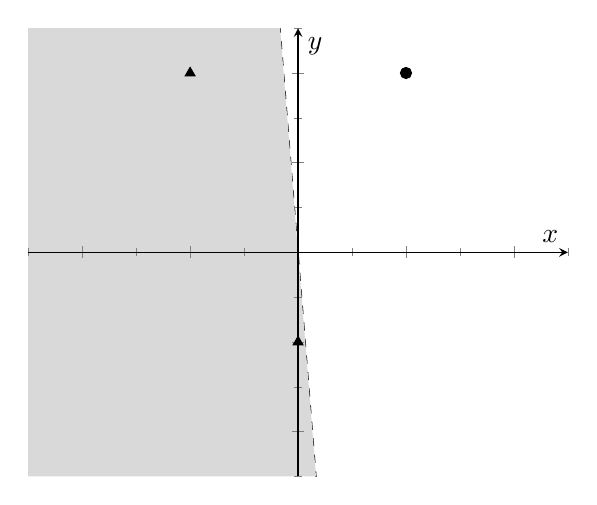
\begin{tikzpicture}
				\begin{axis}[ymin = -2.5, ymax = 2.5, xmax = 2.5, xmin = -2.5, xticklabel = \empty, yticklabel = \empty, minor tick num = 1, axis lines = middle, xlabel = $x$, ylabel = $y$, axis on top]
					\addplot[only marks, mark = *] coordinates {(1, 2)};
					\addplot[only marks, mark = triangle*] coordinates {(-1, 2) (0, -1)};
					\addplot[domain = -3:3, samples = 2, dashed] {-15*x};
					\draw[fill = gray!30, draw = none] (axis cs:-2.5, -2.5) -- (axis cs:-2.5, 2.5) -- (axis cs: -1/6, 2.5) -- (axis cs:1/6, -2.5);
				\end{axis}
			\end{tikzpicture}
			\caption{Puntos separados en $\mathbb{R}^2$}
			\label{fig:separated_label_data}
		\end{figure}
		
		\begin{table}[H]
			\centering
			\begin{tabular}{|c|c|c|}\hline
				$x$ & $y$ & $x \oplus y$\\\hline
				0 & 0 & 0\\\hline
				0 & 1 & 1\\\hline
				1 & 0 & 1\\\hline
				1 & 1 & 0\\\hline
			\end{tabular}
			\caption{Función XOR}
			\label{table:xor}
		\end{table}
		
		\begin{figure}
			\centering
			\begin{tikzpicture}
				\begin{axis}[ymin = -.5, ymax = 2.5, xmax = 2.5, xmin = -.5, xticklabel = \empty, yticklabel = \empty, minor tick num = 1, axis lines = middle, xlabel = $x$, ylabel = $y$]
					\addplot[only marks, mark = *] coordinates {(0, 0) (1, 1)};
					\addplot[only marks, mark = triangle*] coordinates {(0, 1) (1, 0)};
				\end{axis}
			\end{tikzpicture}
			\caption{Valores de $x \oplus y$ en  $\mathbb{R}^2$}
			\label{fig:xor}
		\end{figure}
		
		En cuanto a la pregunta de cómo hallar los parámetros, se consideran las siguientes ecuaciones, donde $\textbf{w}$ es el vector de pesos, $t$ el valor esperado, y $a$ la salida del perceptrón y se aplica el \Cref{algo:perceptron} para obtener los parámetros óptimos. En dicho algoritmo se supondrá que existe una matriz $X$ de $n$ filas que contiene los diferentes $\textbf{x}$. 
		
		$$
		\begin{gathered}
			\textbf{w}(k+1) = \textbf{w}(k) + e(k)\textbf{x}(k)\\
			b(k+1) = b(k) + e(k)\\
			e(k) = t(k) - a(k)\\
			a(k) = u(\textbf{w}^t(k)\textbf{x}(k))
		\end{gathered}
		$$
		
		\begin{algorithm}
			\SetProgSty{texttt}\DontPrintSemicolon
			
			\caption{Regla de aprendizaje del perceptrón}
			\label{algo:perceptron}
			
			\Datos{$X, \textbf{t}$}
			\Resultado{$\textbf{w}, b$}
			$b \gets 0$\\
			$\textbf{w} \gets$ \texttt{random}\\
			$k \gets 0$\\
			\Repetir{$\lnot$\texttt{acabar}}{
				\texttt{acabar} $\gets$ \texttt{true}\\
				\Para{$i \gets k$ \KwTo $k + n - 1$}{
					$e(i) \gets t(i) - a(i)$\\
					$\textbf{w}(i+1) \gets \textbf{w}(i) + e(i)\textbf{x}(i \pmod n)$\\
					$b(i+1) \gets b(i) + e(i)$\\
					\texttt{acabar} $\gets$ \texttt{acabar} $\land \, e(i) == 0$ 
				}
				$k \gets k + n - 1$
			}
		\end{algorithm}
		
		A cada una de las iteraciones que realiza el bucle exterior se les denomina épocas o \textit{epoch}, que consiste en realizar el proceso de entrenamiento sobre todo el conjunto de datos. En este caso se está suponiendo que no va a recibir casos que no sean linealmente separables, pero de lo contrario se puede añadir un contador \texttt{max\_epochs} y fijar un número máximo para no caer en un bucle infinito. No sería tarea fácil determinar dicho valor, pues aunque el algoritmo converge en los casos previamente explicados, no en todos lo hace de manera rápida. A continuación se muestra cómo obtener la solución de la \Cref{fig:separated_label_data}. 
		
		$$
		X = \begin{pmatrix}
			1 & -1 & 0\\
			2 & 2 & -1
		\end{pmatrix} \,\,\, \textbf{t} = \begin{pmatrix}
		1 & 0 & 0
		\end{pmatrix} \,\,\, \textbf{w} = \begin{pmatrix}
		1\\-0.8 \end{pmatrix}
		$$
		
		\begin{enumerate}[label = \textbf{\arabic*. }]
			\item \begin{itemize}
				\item $a(1) = u\left(\begin{pmatrix}1 &-0.8 \end{pmatrix}\begin{pmatrix}
					1\\2 \end{pmatrix}\right) = 0$
				\item $e(1) = t(1) - a(1) = 1 - 0$
				\item $\textbf{w}(2) = \textbf{w}(1) + e(1)\textbf{x}(1) = \begin{pmatrix}
					1\\-0.8 \end{pmatrix} + \begin{pmatrix} 1\\2 \end{pmatrix} = \begin{pmatrix}
					2\\1.2 \end{pmatrix}$
			\end{itemize}
		\end{enumerate}
		
	\chapter{Optimización del proceso de valoración de puntos de interés}

	Después de analizar diversos modelos de aprendizaje automático, junto con sus características y los algoritmos asociados, se ofrece un ejemplo práctico que ilustra la aplicación de estos modelos para abordar un problema de la vida real y buscar una solución adecuada. Para ello se presenta la compañía Niantic, fundada en 2010 como parte de una startup de Google, que se especializa en el desarrollo de juegos para dispositivos móviles que utilizan realidad aumentada (AR). Algunas de sus creaciones más destacadas han sido los juegos Ingress y Pokémon GO. \\
	
	Una de las herramientas creadas por esta empresa es Niantic Lightship, que permite a desarrolladores Unity integrar realidad aumentada y mapas con puntos de interés basados en la ubicación real del jugador. Dado que para Niantic resultaba inviable marcar dichos puntos de interés alrededor de todo el mundo, creó Niantic Wayfarer. En esta herramienta, usuarios experimentados de sus juegos pueden hacer propuestas de puntos de interés (llamados Wayspots) para que de manera colaborativa, otros usuarios las valoren. Sin embargo, tras varios años desde su lanzamiento, debido al gran número de propuestas y al reducido número de valoradores, la comunidad notifica largos tiempos de espera en el proceso de valoración de las propuestas. Por este motivo, se propone en este proyecto realizar una primera aproximación a la automatización de este proceso mediante las técnicas de visión e inteligencia artificial presentadas en el marco teórico. \\
	
	La valoración de un Wayspot en Wayfarer consta de diferentes etapas. En primer lugar se muestra un título y descripción del Wayspot junto con la imagen que aparecería en los juegos. Además aparece una imagen secundaria con una visión desde otra perspectiva, junto con otro texto que ayudarían al valorador a ubicar la propuesta, tal y como se muestra en la \Cref{fig:info_propuesta}. También aparece un breve cuestionario con una serie de preguntas genéricas que ayudan a determinar si aquello que se solicita cumple una serie de criterios (\Cref{fig:preguntas}). Además, se muestra un mapa que contiene los Wayspots cercanos para verificar que no exista ya, y comprobar con Street View la ubicación sugerida (\Cref{fig:mapa}). Finalmente, se pide clasificar la propuesta en una o varias categorías. 
	
	\begin{figure}[!h]
		\centering
		\includegraphics[scale = .4, valign = c]{info_principal}\hfill
		\includegraphics[scale = .4, valign = c]{imagen_principal}\hfill
		\includegraphics[scale = .4, valign = c]{imagen_secundaria}
		\caption{Información de una propuesta en Wayfarer}
		\label{fig:info_propuesta}
	\end{figure}
	
	\begin{figure}[!h]
		\centering
		\includegraphics[scale = .3]{cuestionario}
		\caption{Cuestionario de una propuesta en Wayfarer}
		\label{fig:preguntas}
	\end{figure}
	
	\begin{figure}[!h]
		\centering
		\includegraphics[scale = .3, valign = c]{mapa}\hfill
		\includegraphics[scale = .3, valign = c]{etiquetas}
		\caption{Mapa y clasificación de una propuesta de Wayfarer}
		\label{fig:mapa}
	\end{figure}
	
	\section{Tecnologías empleadas}
	
		\subsection{Python}
		
			Para realizar la codificación del proyecto se ha utilizado el lenguaje de programación Python. Es un lenguaje de alto nivel en el que se pueden seguir diferentes paradigmas de programación, como por ejemplo, el orientado a objetos o el funcional. Sus dos grandes ventajas son su sintaxis, que es muy sencilla y legible; y la gran variedad de bibliotecas que posee para realizar cualquier tipo de tareas, desde desarrollo web, proyectos de aprendizaje automático, desarrollo de videojuegos, creación de animaciones, etc. \\
			
			\begin{figure}[!h]
				\centering
				\includesvg{python}
				\caption{Python}
				\label{fig:py}
			\end{figure}
			
			Para este proyecto, las principales utilizadas son TensorFlow y Scikit-learn. La primera de ellas fue creada por Google y permite construir de manera sencilla modelos de aprendizaje automático, contando con las implementaciones de los principales elementos que los forman, así como algoritmos de entrenamiento, datasets de ejemplo, y funciones auxiliares de utilidad para trabajar con los datos empleados durante el proceso. La segunda de ellas, además de contar también con diversas implementaciones de modelos y algoritmos de aprendizaje automático, es bien conocida por contar con las implementaciones de diferentes métricas para modelos, lo que permite comprobar de manera rápida y visual la calidad de los modelos entrenados. Finalmente, estas bibliotecas hacen uso de otras como pueden ser Matplotlib, utilizada para generar cualquier tipo de figura desde Python. \\
			
			\begin{figure}[!h]
				\centering
				\begin{subfigure}{.5\textwidth}
					\centering
					\includesvg{tf}
					\caption{TensorFlow}
					\label{fig:tf}
				\end{subfigure}\hfill
				\begin{subfigure}{.5\textwidth}
					\centering
					\includesvg[scale = .7]{sklearn}
					\caption{Scikit-learn}
					\label{fig:sklearn}
				\end{subfigure}
				\caption{Bibliotecas populares de Python}
				\label{fig:bibliotecas}
			\end{figure}
			
			Por otro lado, no todo son ventajas. Python es un lenguaje interpretado y de tipado dinámico, lo que hace que su ejecución sea mucho más lenta que la de otros lenguajes. Sin embargo, existen soluciones como NumPy, una biblioteca que permite trabajar con grandes matrices de datos en tiempos de ejecución menores que al utilizar listas, gracias a que gran parte de su codificación se realizó utilizando lenguajes de más bajo nivel como C. 
		
		\subsection{CUDA}
		
			CUDA son las siglas de Compute Unified Device Architecture, y es una tecnología de la marca estadounidense NVIDIA. Esta tecnología hace referencia a un conjunto de elementos que permiten ejecutar código de manera masivamente paralela en una tarjeta gráfica de la compañía, de manera que el tiempo de ejecución es mucho menor que al ejecutarlo de manera secuencial. Entre estos elementos se encuentran el controlador, el compilador, las interfaces para los diferentes lenguajes (la más común la de C/C++), las librerías que contienen algoritmos optimizados, y los propios núcleos CUDA de la GPU\cite{cuda}. \\
			
			\begin{figure}[!h]
				\centering
				\includesvg[width = .3\textwidth]{nvidia}
				\caption{NVIDIA}
				\label{fig:nvidia}
			\end{figure}
			
			El hardware de las tarjetas gráficas de NVIDIA se divide en \textit{streaming multiprocessors} (SMs), que a su vez están compuestos de \textit{streaming processors} (SPs) o núclos CUDA, entre otros elementos. A nivel de software, la unidad básica paralela es el hilo, que a nivel de hardware se ejecuta en un SP. Dichos SPs, son unos núcleos capaces de hacer operaciones más sencillas que las que un núcleo de una CPU podría realizar, pero de manera más rápida. A su vez, los hilos se agrupan en bloques, teniendo en cuenta que a nivel de hardware cada bloque se ejecuta en un único SM. Finalmente, todos los elementos se agrupan en una cuadrícula (o \textit{grid}) compuesta de bloques. Cada cuadrícula se ejecuta en una única GPU a nivel de hardware, y ejecuta a nivel de software un kernel\cite{cuda_arq,cuda_arq1}. \\
			
			\begin{figure}[!h]
				\centering
				\includegraphics[scale = .3]{arquitectura_cuda}
				\caption{Arquitectura CUDA a nivel de hardware y software\cite{cuda_arq1}}
				\label{fig:arq_cuda}
			\end{figure}
			
			El hecho de poder realizar miles de operaciones sencillas de manera simultánea, reduce enormemente el tiempo de ejecución de algoritmos que son paralelizables, es decir, que contienen pasos sencillos que son independientes de otros y se pueden realizar al mismo tiempo, como es el caso de una convolución o multiplicación de matrices. Además, se cuenta con diferentes niveles de memoria, con los que se agilizan los tiempos de lectura de elementos que son utilizados frecuentemente. \\
			
			La mayoría de algoritmos de aprendizaje automático de TensorFlow tienen implementada su versión paralela, de manera que si se cuenta con una GPU compatible con CUDA, TensorFlow la utilizará para ahorrar el mayor tiempo posible durante los entrenamientos de los modelos. En este caso se dispone de un equipo que cuenta con un procesador Intel Core i7-8700, una GPU NVIDIA GeForce GTX 1060 6GB, y 32 GB de RAM; lo que hace posible la ejecución concurrente de dichos algoritmos. Esta tarjeta gráfica cuenta con 1280 SPs o núcleos CUDA repartidos en 10 SMs. \\
			
			Si bien el trabajo de indicar a TensorFlow que haga uso de CUDA es sencillo, no es tan trivial la configuración de drivers de NVIDIA, instalación de CUDA, versión de Python, versión de TensorFlow, versión de sistema operativo, etc. Con el frecuente cambio de versiones de cada componente, se presentan nuevas incompatibilidades entre ellos, haciendo que guías oficiales fallen y que el proceso de configuración inicial sea complicado en sistemas operativos como Windows 11. La manera más sencilla actualmente de realizar una instalación de CUDA y TensorFlow es sobre el sistema operativo Ubuntu en su versión 22.04 LTS. Para instalar y configurar el resto de componentes se ha hecho uso de LambdaStack (\url{https://lambdalabs.com/lambda-stack-deep-learning-software}). Mediante el uso del comando de terminal
			\begin{verbatim}
				wget -nv -O- https://lambdalabs.com/install-lambda-stack.sh | sh -
			\end{verbatim}
			automáticamente lanza LambdaStack que se encarga de instalar las versiones de Python y sus librerías (TensorFlow y PyTorch entre otras) adecuadas, los drivers de NVIDIA correctos, componentes de CUDA, realiza las configuraciones de variables de entorno, etc. En general, deja el entorno de Ubuntu configurado para poder trabajar en cualquier proyecto de inteligencia artificial en el que se quiera hacer uso de una GPU de NVIDIA. También cuentan con una imagen de Docker que ofrece una experiencia similar. El uso de este servicio es completamente gratuito, y es el que utiliza la compañía que lo gestiona en sus servicios de cloud computing (que sí son de pago). \\
			
			Para probar la eficacia del uso de CUDA para proyectos de esta índole, se ha seleccionado un modelo de los que se presentan en la \Cref{subsec:crear_cnn} (entrenamiento de una red convolucional desde cero), y se ha lanzado midiendo el tiempo, el mismo entrenamiento pero con diferente número de épocas sobre CPU y GPU. La \Cref{fig:comparativa_cuda} evidencia cómo el entrenamiento en la GPU llega a ser hasta cinco veces más rápido que en la CPU. Todos los entrenamientos de la \Cref{subsec:crear_cnn} han sido realizados sobre la GPU. 
			
			\begin{figure}[!h]
				\centering
				\includegraphics[scale = .5]{comp_cuda}
				\caption{Comparativa de entrenamiento en CPU frente a en GPU}
				\label{fig:comparativa_cuda}
			\end{figure}
			
		\subsection{Google Cloud Platform}
		
			Google Cloud Platform o GCP es una de las plataformas de cloud computing más conocidas, junto con Amazon Web Services (AWS) y Microsoft Azure. Este tipo de plataformas se encargan de ofrecer servicios IaaS (infraesctructura como servicio), PaaS (plataforma como servicio), y SaaS (software como servicio) muy útiles para empresas a la hora de desarrollar todo tipo de proyectos. Google divide los tipos de servicios que ofrece en diferentes categorías, siendo algunas de las principales las siguientes \cite{gcp}.  
			
			\begin{itemize}
				\item Inteligencia artificial y aprendizaje automático: GCP cuenta con una amplia gama de servicios de inteligencia artificial en sus distintas áreas como por ejemplo, procesamiento de lenguaje, visión artificial, IA generativa, etc. Su plataforma Vertex AI engloba una gran variedad de modelos muy útiles y permite entrenar, desplegar, y gestionar dichos modelos de manera sencilla. En general, se podrían categorizar como servicios PaaS y SaaS. 
				\item Inteligencia empresarial: Google ofrece herramientas (SaaS) como podrían ser Looker y Looker Studio, que permiten trabajar con datos, analizarlos, visualizarlos, generar informes, y en general, todo tipo de tareas del campo de Business Intelligence. 
				\item Computación: dentro de este campo Google ofrece diferentes variantes de hardware virtualizado, como por ejemplo, máquinas virtuales, GPUs, ejecución de aplicaciones en contenedores, etc. En resumen, se trata de diferentes servicios IaaS y PaaS
				\item Bases de datos y almacenamiento: Google ofrece múltiples servicios de almacenamiento de ficheros y bases de datos tanto SQL como NoSQL, de manera segura y escalable. De manera similar al apartado anterior, son principalmente servicios IaaS y PaaS. 
			\end{itemize}
			
			La mayoría de estos servicios son accesibles de manera sencilla vía CLI, API, o los diferentes SDK de los lenguajes de programación más populares. 
			
			\begin{figure}[!h]
				\centering
				\includegraphics[scale = .2]{gcp}
				\caption{Google Cloud Platform}
				\label{fig:gcp}
			\end{figure}
			
			

	\section{Clasificación de imágenes mediante redes convolucionales}
	
		Una primera aproximación a agilizar el proceso de valoración comentado, sería detectar el objeto que se muestra en la imagen de la propuesta, para que en caso de que sea algo aceptable proseguir con el proceso de valoración, o en caso contrario, rechazar directamente la propuesta. En general, en función del objeto que aparezca en la imagen, se tienen directamente las respuestas a las preguntas de la \Cref{fig:preguntas}. \\
		
		Para comenzar este caso práctico, lo primero a realizar es el proceso conocido como ETL, que consiste en la extracción, transformación, y carga de los datos; para posteriormente poder trabajar con ellos y proporcionárselos al modelo. Comenzando por la extracción de datos, se presenta el primero de los problemas. La idea es utilizar imágenes que realmente hayan pasado por este proceso de valoración para poder hacer el proyecto lo más realista posible, sin embargo, ni Wayfarer ni ninguno de los juegos poseen alguna API (al menos de manera pública) que permita recolectar de manera programática las imágenes utilizadas o información relativa a ellas. 
		
		\subsection{Proceso ETL}
		
			La solución adoptada para este proceso, ha sido recolectar manualmente imágenes que han superado el proceso de valoración, pudiendo consultar algunas de ellas desde el mapa de uno de los juegos (\url{https://intel.ingress.com/}). En este caso, se estarían clasificando entre las $n$ clases de objetos aceptables las imágenes recibidas, cosa que en un primer momento parece carecer de sentido pues se conoce el resultado de la valoración. Sin embargo, al no tener acceso a propuestas rechazadas, no se pueden recolectar estos datos para entrenar los modelos, pero si de la empresa responsable se tratase, se dispondría de una enorme cantidad de imágenes válidas y no válidas etiquetadas (gracias a la parte del proceso de valoración que muestra la \Cref{fig:mapa}), y que se podrían cargar de manera automática. En resumen, cambiando simplemente los datos que se cargarían y su fuente, se podrían tomar las siguientes decisiones sin necesidad de modificar el resto del proyecto.  
			
			\begin{itemize}
				\item Si $I \in C_i, 0 \leq i < m$, rechazar la propuesta
				\item Si $I \in C_j, m \leq j < n$, continuar evaluando la propuesta
			\end{itemize}
			
			Continuando con la extracción de los datos, y preparándolos para la carga, se ha creado una carpeta \texttt{tfg\_dataset} que representa el conjunto de las imágenes que se utilizan durante el proyecto. Dentro de esta, se ubicarán dos subcarpetas, \texttt{train} y \texttt{test}, que hacen referencia a las imágenes que se utilizarán para entrenar los modelos, y las que se utilizarán para evaluar su rendimiento. Para generar dichas carpetas partiendo de una que contiene las imágenes separadas por clases, se ha codificado la función \texttt{split\_tt} que permite hacer la división del conjunto en los de entrenamiento y test con el porcentaje especificado. Previamente a la ejecución de esta función, se recomienza ejecutar otra que se ha codificado llamada \texttt{renombrar\_imagenes}, que dada la ruta raíz donde se encuentran las carpetas de cada clase, renombra las imágenes de cada carpeta de manera que queden enumeradas. Esta es la manera de etiquetar el conjunto de datos y prepararlo para la carga. Se puede visualizar un breve esquema de esta estructura en la \Cref{fig:arbol_dataset}. \\
			
			\begin{figure}[!h]
				\centering
				\scriptsize
				\Tree[.\texttt{tfg\_dataset} [.\texttt{train} [.\texttt{clase\_1} $\vdots$ ] [.\texttt{clase\_2} \texttt{0.jpg} $\cdots$ \texttt{22.jpg} ] $\cdots$ [.\texttt{clase\_n} $\vdots$ ] ] [.\texttt{test} [.\texttt{clase\_1} $\vdots$ ] [.\texttt{clase\_2} \texttt{10.jpg} $\cdots$ \texttt{33.jpg} ]  $\cdots$ [.\texttt{clase\_n} $\vdots$ ] ] ]
				\caption{Árbol de carpetas del dataset}
				\label{fig:arbol_dataset}
			\end{figure}
			
			Para cargar el dataset en TensorFlow directamente desde la estructura de carpetas creadas, se hará uso de la función \texttt{image\_dataset\_from\_directory} de \texttt{utils}. Esta contiene una serie de parámetros interesantes a comentar. 
			
			\begin{itemize}
				\item \texttt{directory}: es el directorio raíz del dataset, en este caso \texttt{tfg\_dataset}. 
				\item \texttt{image\_size}: es una tupla de dos elementos con las dimensiones en píxeles que deberán tener las imágenes del dataset. 
				\item \texttt{labels}: mediante el valor \texttt{inferred} las etiquetas toman el mismo valor que el nombre de las carpetas. 
				\item \texttt{label\_mode}: hace referencia a la forma de codificar las etiquetas. Se empleará el valor \texttt{categorical} para codificar las etiquetas utilizando one-hot-encoding, es decir, si se tienen por ejemplo cuatro clases y un elemento pertenece a la cuarta, dicha etiqueta queda codificada como 0001. 
				\item \texttt{batch\_size}: hace referencia al tamaño de batch o lote que será utilizado durante el entrenamiento. Si en la función de entrenamiento se elige un tamaño diferente, se utilizará el menor de los valores. 
				\item \texttt{validation\_split}: hace referencia al porcentaje de los datos de entrenamiento que se reservan para validar el modelo durante el entrenamiento, es decir, permiten calcular el error del modelo al hacer una predicción de datos que nunca ha visto mientras entrena. Se reservarán un 20\% de los datos para validar. 
				\item \texttt{seed}: hace referencia a la semilla que se utiliza para ordenar las imágenes de manera aleatoria. 
				\item \texttt{subset}: seleccionando el valor \texttt{both} permite devolver el conjunto de entrenamiento y validación con la llamada a la función, es decir, \texttt{x\_train, x\_val = image\_dataset\_from\_directory(...)}. 
			\end{itemize}
			
			Como se puede observar, esta función que está haciendo principalmente el trabajo de la carga de datos, también hace parte del proceso de transformación, ya que permite modificar las dimensiones de la imagen (en este caso se utilizará un valor de $224 \times 224$ píxeles, se justificará más adelante), y también permite modificar la codificación de las etiquetas. Además, cada píxel (en cada canal de color) toma un valor entre 0 y 255. Es muy importante normalizar estos valores en el proceso de transformación para facilitar el trabajo a los diferentes modelos. Para ello, con ayuda de una capa de reescalado de Keras, se divide el valor de cada píxel entre 255 para obtener valores entre 0 y 1. Con motivo de verificar que todos estos pasos se han realizado correctamente, se codificado una función llamada \texttt{sample\_ds\_dfd} que permite visualizar nueve ejemplos aleatorios de un dataset creado con la función de TensorFlow mencionada, obteniendo como resultado la \Cref{fig:sample_dataset}. \\
			
			\begin{figure}
				\centering
				\includegraphics[scale = .8]{sample_dataset}
				\caption{Visualización de ejemplo de un dataset creado}
				\label{fig:sample_dataset}
			\end{figure}
			
		\subsection{Creación y entrenamiento de una red convolucional en TensorFlow}\label{subsec:crear_cnn}
		
			En esta primera aproximación se va a crear y entrenar una red convolucional desde cero con el dataset mencionado. En este caso, se han elegido cuatro tipos de objetos que frecuentemente se proponen como puntos de interés: parques infantiles, carteles informativos, marcadores de ruta, e hitos del Camino de Santiago. Mediante la clase \texttt{Sequential} de Keras, se puede proporcionar una lista de las capas que conforman el modelo. La primera de ellas será una capa de convolución, con la particularidad de que se debe indicar el tamaño de entrada, siendo este un tensor de las dimensiones indicadas en la creación del dataset. Se alterna cada capa de convolución ReLU de stride $3 \times 3$ y 32 o 64 filtros, con una capa de maxpooling con stride $2 \times 2$. Estos valores han sido elegidos de manera arbitraria. Esta arquitectura se puede visualizar en la \Cref{fig:arq_cnn}. \\
			
			\begin{figure}[!h]
				\centering
				\includegraphics[scale = .55]{arq_cnn}
				\caption{Arquitectura de la red convolucional}
				\label{fig:arq_cnn}
			\end{figure}
			
			Mediante estas capas, se supone que la red debe extraer características de las imágenes, como por ejemplo
			
			\begin{itemize}
				\item Aparece un objeto rectangular
				\item Tiene dos patas 
				\item No tiene formas curvas
			\end{itemize}
			y de ahí con ayuda de una red clásica, ser capaz de deducir que en la imagen aparece un cartel. En realidad, las capas de convolución no obtienen características tan claras, pero sí resultan con una matriz de detalles en la imagen que pueden conducir a la misma conclusión. Para ello se utiliza la capa \texttt{Flatten} que transforma dicha matriz en un vector que sirve de entrada a la siguiente y última capa de la red, una capa oculta con tantas neuronas como clases diferentes. Como función de activación se utiliza softmax para obtener una distribución de probabilidad en la que se observe cuál es claramente la clase a la que pertenece el objeto, y con qué confianza lo es. Finalmente, mediante la función \texttt{summary} se puede observar un resumen del modelo. 
			
			\begin{verbatim}
				_________________________________________________________________
				Layer (type)                Output Shape              Param #   
				=================================================================
				conv2d (Conv2D)             (None, 222, 222, 32)      896       
				
				max_pooling2d (MaxPooling2  (None, 111, 111, 32)      0         
				D)                                                              
				
				conv2d_1 (Conv2D)           (None, 109, 109, 64)      18496     
				
				max_pooling2d_1 (MaxPoolin  (None, 54, 54, 64)        0         
				g2D)                                                            
				
				conv2d_2 (Conv2D)           (None, 52, 52, 64)        36928     
				
				max_pooling2d_2 (MaxPoolin  (None, 26, 26, 64)        0         
				g2D)                                                            
				
				flatten (Flatten)           (None, 43264)             0         
				
				dense_2 (Dense)             (None, 8)                 346120    
				
				dense_3 (Dense)             (None, 4)                 36        
				
				=================================================================
				Total params: 402476 (1.54 MB)
				Trainable params: 402476 (1.54 MB)
				Non-trainable params: 0 (0.00 Byte)
				_________________________________________________________________
			\end{verbatim}
			
			Con la función \texttt{compile} se termina de crear el objeto que representa al modelo, pudiendo especificar un optimizador, la función de pérdida, y las métricas que se muestran durante el entrenamiento. Para este proyecto se utilizarán Adam, entropía cruzada, y precisión respectivamente. El modelo ya está en condiciones de ser entrenado, y esto se logra mediante la función \texttt{fit}, a la que se le proporcionan los datos de entrenamiento (\texttt{x\_train}), los datos de validación (\texttt{x\_val}), el número de épocas (en este caso se han elegido 25), y la ruta de los callbacks. Esta sirve para ir almacenando metadatos del entrenamiento, que mediante una utilidad con la que cuenta TensorFlow llamada TensorBoard, permite monitorizar de manera muy visual la calidad del entrenamiento, tal y como se muestra en la \Cref{fig:tb_cnn}. \\
			
			\begin{figure}[!h]
				\centering
				\begin{subfigure}{.4\textwidth}
					\centering
					\includesvg[width = .85\textwidth]{evaluation_loss_vs_iterations_cnn}
					\caption{Iteraciones frente a pérdida}
					\label{fig:tb_cnn_a}
				\end{subfigure}\hfill
				\begin{subfigure}{.4\textwidth}
					\centering
					\includesvg[width = .85\textwidth]{evaluation_accuracy_vs_iterations_cnn}
					\caption{Iteraciones frente a precisión}
					\label{fig:tb_cnn_b}
				\end{subfigure}
				\begin{subfigure}{.4\textwidth}
					\centering
					\includesvg[width = .85\textwidth]{epoch_loss_cnn}
					\caption{Pérdida sobre el conjunto de entrenamiento y validación}
					\label{fig:tb_cnn_c}
				\end{subfigure}\hfill
				\begin{subfigure}{.4\textwidth}
					\centering
					\includesvg[width = .85\textwidth]{epoch_accuracy_cnn}
					\caption{Precisión sobre el conjunto de entrenamiento y validación}
					\label{fig:tb_cnn_d}
				\end{subfigure}
				\caption{Pérdida y precisión durante el entrenamiento de la CNN}
				\label{fig:tb_cnn}
			\end{figure}
			
			La situación que describen las gráficas, es negativa y sería la típica no deseada, pues se observa como con el paso de las iteraciones el error crece mientras que la precisión se estanca en valores no deseados. En concreto, en la \Cref{fig:tb_cnn_c} se observa cómo el error sobre el conjunto de validación crece, mientras que sobre el conjunto de entrenamiento tiende a cero. Esta es una situación denominada como sobreaprendizaje u \textit{overfitting}\cite{overfitting}. La red no tiene capacidad de aprender ni generalizar, y lo que está haciendo es memorizar los datos de ejemplo que se le presentan, cometiendo entonces errores cuando recibe datos que no ha visto nunca. 
			
		\subsection{Transfer learning en TensorFlow}
		
			Como se ha podido observar durante la sección anterior, el resultado del entrenamiento no ha sido adecuado, pues la red tendía a memorizar los datos que se le presentaban sin mostrar una buena capacidad de generalización. Esto puede deberse a múltiples factores, como por ejemplo, que al tener un conjunto de datos de entrenamiento tan reducido no sea capaz de extraer correctamente las características que determinan a los objetos de cada clase. Es decir, en vez de hacerle llegar a las capas densas hechos como ``tiene un objeto rectangular'', ``tiene dos patas'', etc; podría estar haciéndole llegar, ``hay dos árboles en el fondo''. Observando la estructura del modelo, se está tratando de optimizar cerca un millón de parámetros con poco más de 500 observaciones, algo que es muy desproporcionado; la red no es capaz de encontrar relaciones con tan pocos datos. \\
			
			En proyectos similares del mundo real, y en los que además se dispone de pocos datos (como es el caso), es muy poco frecuente crear y entrenar un modelo desde cero tal y como se ha realizado en la \Cref{subsec:crear_cnn}. En vez de realizar esto, es muy común utilizar una técnica conocida como transfer learning. Tal y como se menciona en \cite{transfer}, es una técnica muy aplicada en casos en los que se dispone de pocos datos y los modelos de deep learning no son capaces de encontrar relaciones, y también en casos en los que se dispone de equipos con pocos recursos. Consiste en aplicar el conocimiento obtenido de otro dataset, no necesariamente relacionado, para facilitar el proceso de obtener el conocimiento deseado del dataset actual. \\
			
			En el problema que se está tratando, se va a aplicar esta técnica de la siguiente manera. Como previamente se ha mencionado, las redes convolucionales, pueden verse como un conjunto de capas capaces de extraer características de las imágenes, junto con una red neuronal clásica que es capaz de clasificar en función de dichas características. Teniendo en cuenta que el principal problema del modelo anterior podría ser que no fuera capaz de obtener las características adecuadas que definen a cada clase, la idea es utilizar una serie de capas que sí sean capaces de obtener de manera correcta las características de una imagen, para después poder entrenar la red neuronal clásica con las características adecuadas. \\
			
			Con ayuda de la plataforma TensorHub que trabaja junto con TensorFlow, se pueden importar modelos ya entrenados. En este caso para aplicar la técnica de transfer learning, se ha decidido utilizar la red MobileNet de Google que se observa en la \Cref{fig:mb}. El modelo se puede importar como si de una capa se tratase al crear un modelo secuencial de Keras. Para lograr la técnica, será clave declarar que los parámetros de dicha capa no se deberán entrenar (pues al importar el modelo ya vienen con unos valores adecuados). A continuación se coloca una capa densa, encargada de clasificar las características que la red de Google extraiga, y que deberá ser entrenada. Esta vez, el número de parámetros a optimizar sí es más adecuado al número de observaciones disponibles. 
			
			\begin{figure}[!h]
				\centering
				\includegraphics[scale = .3]{mb}
				\caption{MobileNetV2}
				\label{fig:mb}
			\end{figure}
			
			\begin{verbatim}
				_________________________________________________________________
				Layer (type)                Output Shape              Param #   
				=================================================================
				mobilenetv2_1.00_224 (Func  (None, 7, 7, 1280)        2257984   
				tional)                                                         
				
				global_average_pooling2d (  (None, 1280)              0         
				GlobalAveragePooling2D)                                         
				
				dense_2 (Dense)             (None, 8)                 10248     
				
				dense_3 (Dense)             (None, 4)                 36        
				
				=================================================================
				Total params: 2268268 (8.65 MB)
				Trainable params: 10284 (40.17 KB)
				Non-trainable params: 2257984 (8.61 MB)
				_________________________________________________________________
			\end{verbatim}
			
			La manera de lanzar el entrenamiento es la misma que en el anterior, sin embargo, esta vez los resultados obtenidos son totalmente distintos, tal y como muestran las gráficas de TensorBoard en la \Cref{fig:tb_tl}. \\
			
			\begin{figure}[!h]
				\centering
				\begin{subfigure}{.4\textwidth}
					\centering
					\includesvg[width = .85\textwidth]{evaluation_loss_vs_iterations_mb}
					\caption{Iteraciones frente a pérdida}
					\label{fig:tb_tl_a}
				\end{subfigure}\hfill
				\begin{subfigure}{.4\textwidth}
					\centering
					\includesvg[width = .85\textwidth]{evaluation_accuracy_vs_iterations_mb}
					\caption{Iteraciones frente a precisión}
					\label{fig:tb_tl_b}
				\end{subfigure}
				\begin{subfigure}{.4\textwidth}
					\centering
					\includesvg[width = .85\textwidth]{epoch_loss_mb}
					\caption{Pérdida sobre el conjunto de entrenamiento y validación}
					\label{fig:tb_tl_c}
				\end{subfigure}\hfill
				\begin{subfigure}{.4\textwidth}
					\centering
					\includesvg[width = .85\textwidth]{epoch_accuracy_mb}
					\caption{Precisión sobre el conjunto de entrenamiento y validación}
					\label{fig:tb_tl_d}
				\end{subfigure}
				\caption{Pérdida y precisión durante el entrenamiento aplicando transfer learning}
				\label{fig:tb_tl}
			\end{figure}
			
			Estas gráficas representan una situación cercana a la ideal. En las \Cref{fig:tb_tl_a,fig:tb_tl_b} se observa cómo con el paso de las iteraciones, el error disminuye y la precisión aumenta hasta llegar a valores adecuados. Además, en las \Cref{fig:tb_tl_c,fig:tb_tl_d} se muestra claramente que tanto el error como la precisión se comportan de manera similar sobre los conjuntos de entrenamiento y validación respectivamente, tomando además valores adecuados. 
			
		\subsection{Aumento de datos}
		
			Como se ha visto a lo largo de las secciones anteriores, uno de los problemas que se está teniendo en este caso práctico, es la falta de datos. Una técnica utilizada frecuentemente en estos casos es conocida como aumento de datos. Consiste en modificar las imágenes del dataset de entrenamiento para que el modelo disponga de más ejemplos diferentes\cite{augm}. Podría entenderse como una parte del proceso de transformación ETL. \\
			
			Una vez más, es posible aplicar esta técnica mediante funciones de TensorFlow. Para ello se crea un objeto de la clase \texttt{ImageDataGenerator}. Mediante su constructor se pueden declarar los valores que toman los atributos que modificarán las imágenes, siendo algunos de los más destacables: 
			
			\begin{itemize}
				\item \texttt{rotation\_range}: gira la imagen. 
				\item \texttt{width\_shift\_range} y \texttt{height\_shift\_range}: desplazamiento horizontal y vertical de la imagen. 
				\item \texttt{shear\_range}: estira la imagen. 
				\item \texttt{zoom\_range}: hace zoom a la imagen. 
				\item \texttt{reescale}: indica el factor por el que se reescala la imagen, en este caso $1/255$ para facilitar el entrenamiento a la red, como en casos anteriores. 
				\item \texttt{validation\_split}: porcentaje de los datos reservados a validación. 
			\end{itemize}
			
			Una vez se tiene declarado el generador, se utiliza su método \texttt{flow\_from\_directory} para que dada la ruta que contiene las imágenes, el tamaño deseado de imagen, y el tamaño de los lotes, se cree el objeto que representa al dataset. De manera similar a la anterior, se ha programado una función \texttt{sample\_ds\_ffd} que permite visualizar nueve elementos del dataset creado, tal y como muestra la \Cref{fig:sample_dataset_au}. Esta es una de la manera más común de crear datos nuevos, siendo alguna de las más novedosas las arquitecturas GAN. Están formadas por dos redes, una capaz de crear imágenes y otra capaz de distinguir entre imágenes reales y generadas, y transmitir dicho conocimiento a la primera red, de manera que una intente ``engañar'' a la otra\cite{gan}. \\
			
			\begin{figure}
				\centering
				\includegraphics[scale = .8]{sample_dataset_au}
				\caption{Visualización de ejemplo de un dataset aplicando aumento de datos}
				\label{fig:sample_dataset_au}
			\end{figure}
			
			Contando ahora con el dataset original y el modificado, la técnica del aumento de datos se puede aplicar de dos formas. La primera de ellas es crear un modelo y entrenar únicamente con el datset modificado. Esto puede dar una mayor capacidad de generalización al modelo al mostrar imágenes más diferentes de objetos similares. La segunda de ellas consiste en entrenar el modelo con el dataset original, y después con el dataset modificado (sin cambiar qué imágenes pertenecen a los conjuntos de entrenamiento, validación, y test en cada dataset). Esta puede dar mejores resultados, pues tiene más observaciones y el modelo puede de ver el mismo objeto ``de diferentes formas''. Sin embargo hay que tener cuidado con esta segunda opción, pues podría conducir a situaciones de sobreajuste. 
			
		\subsection{Evaluación de los modelos}
		
			Si bien gracias a las gráficas que TensorBoard proporciona es posible hacerse una idea de la calidad que tendrán las predicciones de un modelo, no son suficientes. Será entonces el momento de presentar al modelo una serie de imágenes que nunca haya visto para poder evaluar la calidad de sus predicciones mediante una serie de métricas y valores estadísticos. Este conjunto de imágenes que el modelo no ha recibido hasta el momento, es el denominado conjunto de test. \\
			
			Para calcular estas métricas en Python, se va a utilizar la librería Scikit-learn, ya que contiene un conjunto de métodos con los que calcular y visualizar la mayoría de métricas empleadas en machine learning. Además, las predicciones sobre los conjuntos de test quedará representadas mediante dos matrices, \texttt{Y\_matrix} y \texttt{Y\_score}. La primera de ellas es una matriz $n \times 3$ que contiene para cada observación su etiqueta real, la predicha, y con qué probabilidad se le asigna. La segunda, contiene las probabilidades de cada observación de pertenecer a cada clase, por tanto es de dimensiones $n \times c$. 
			
			\begin{align*}
				Y_m &= \begin{pmatrix}
					0 & 0 & 0.75\\
					2 & 2 & 0.7\\
					3 & 1 & 0.97\\
					\vdots & \vdots & \vdots\\
					1 & 1 & 0.87
				\end{pmatrix} & 
				Y_s &= \begin{pmatrix}
					0.75 & 0.07 & 0.01 & 0.17\\
					0.15 & 0.01 & 0.7 & 0.14\\
					0.02 & 0.97 & 0.01 & 0.01\\
					\vdots & \vdots & \vdots & \vdots\\
					0.05 & 0.87 & 0.01 & 0.08
				\end{pmatrix}
			\end{align*}
			
			Dependiendo si el problema en cuestión es de regresión o clasificación, se deben utilizar unas métricas u otras. Debido a que se desea evaluar la calidad de una clasificación, se han elegido las siguientes. 
			
			\subsubsection{Matriz de confusión}\label{subsub:matriz_confusion}
			
				La matriz de confusión muestra en el caso de clasificación binaria, los verdaderos positivos, verdaderos negativos, falsos positivos, y falsos negativos, mientras que en el caso de clasificación no binaria, en general la relación entre las etiquetas reales de cada observación y las que el modelo le ha asignado\cite{confusion}. De manera muy visual se puede observar la cantidad de ejemplos de cada clase (pudiendo ver si se encuentran desbalanceadas), cuántos han sido clasificados correctamente, cuántos no, y en general entre qué clases suele confundirse más el modelo. \\
				
				\begin{figure}[!h]
					\centering
					\begin{subfigure}{.4\textwidth}
						\centering
						\includegraphics[scale = .34]{mc_conv}
						\caption{Normal}
						\label{fig:mc_conv}
					\end{subfigure}\hfill
					\begin{subfigure}{.4\textwidth}
						\centering
						\includegraphics[scale = .34]{mc_mb}
						\caption{Aplicando transfer learning}
						\label{fig:mc_mb}
					\end{subfigure}
					\begin{subfigure}{.4\textwidth}
						\centering
						\includegraphics[scale = .34]{mc_convau}
						\caption{Aplicando aumento de datos}
						\label{fig:mc_convau}
					\end{subfigure}\hfill
					\begin{subfigure}{.4\textwidth}
						\centering
						\includegraphics[scale = .34]{mc_mbau}
						\caption{Aplicando ambas}
						\label{fig:mc_mbau}
					\end{subfigure}
					\caption{Matrices de confusión}
					\label{fig:mc}
				\end{figure}
				
				En la \Cref{fig:mc} se observan las matrices de confusión de las cuatro situaciones descritas anteriormente. El elemento $a_{ij}$ representa la cantidad de observaciones de la clase $C_i$ que han sido clasificadas como $C_j$ (a partir de ahora, $\hat{C}_j$). La situación ideal se da cuando en el caso de que $i \neq j$, entonces $a_{ij} = 0$, o lo que es lo mismo, que solo haya valores  en la diagonal principal, pues a todos se les estaría asignando la clase correcta. Además, en esta representación gráfica sería deseable que todos los elementos de dicha diagonal tuviesen el mismo color, pues la situación actual describe un desbalanceo entre las clases. Se ve claramente que al aplicar transfer learning (\Cref{fig:mc_mb,fig:mc_mbau}) se obtienen resultados mucho mejores que al entrenar el modelo desde cero, tal y como las curvas de TensorBoard parecían indicar, pues la cantidad de malas clasificaciones es muy pequeña. La diferencia en dicho caso entre usar aumento de datos o no, no es muy significativa. \\
				
				Para poder calcular la matriz de confusión, se ha utilizado la función \texttt{confusion\_matrix} de Scikit-learn, que recibe como parámetros un vector con las clases reales de cada observación, y otro con las que el modelo les ha asignado. Mediante la función \texttt{ConfusionMatrixDisplay} se puede ver de manera gráfica la matriz (\Cref{fig:mc}). Con diferentes parámetros se pueden cambiar los colores e incrustar código \LaTeX{} para modificar los textos. Se ha codificado la función \texttt{matriz\_confusion} que recibe el dataset y $Y_m$, y muestra el gráfico con la configuración personalizada. 
				
			\subsubsection{Precisión, sensibilidad, y $F_1-$score}\label{subsub:f1}
				
				Si bien la matriz de confusión permite mostrar de manera visual la calidad de las clasificaciones, es conveniente calcular algunos valores \cite{metricas_matriz} a partir de esta matriz que permitan visualizar de manera numérica dichas calidades. La primera de ellas conocida como \textbf{precisión} $(\mathcal{P})$, y puede entenderse como la probabilidad de que un elemento que etiquetado como $C_i$, realmente pertenezca a dicha clase. 
				
				$$
				\mathcal{P} = P(C_i | \hat{C}_i) = \frac{P(C_i \cap \hat{C}_i)}{P(\hat{C}_i)}
				$$
				
				La siguiente se denomina \textbf{sensibilidad} (o recuerdo, $\mathcal{R}$) e indica la probabilidad de que un elemento de la clase $C_i$, se clasifique como tal. 
				
				$$
				\mathcal{R} = P(\hat{C}_i | C_i) = \frac{P(\hat{C}_i \cap C_i)}{P(C_i)}
				$$
				
				En resumen y en términos de probabilidad condicionada, $\mathcal{P}$ puede entenderse como una probabilidad a posteriori (cómo de bien ha clasificado el modelo), mientras que $\mathcal{R}$ puede entenderse como una probabilidad a priori (cómo de bien clasificaría el modelo). Es frecuente calcular la media armónica de estos dos valores para obtener un único valor que evalúe la calidad de clasificación del modelo, comúnmente llamada $F_1$. 
				
				$$
				F_1 = \frac{2}{\mathcal{P}^{-1} + \mathcal{R}^{-1}}
				$$
				
				Para calcular estos valores, se ha hecho uso de la función \texttt{classification\_report} de Scikit-learn, que muestra en una tabla estos valores para cada clase, junto con las medias de dichos valores. En situaciones de clases desbalanceadas como es esta, es conveniente mirar las medias ponderadas (\texttt{weighted avg}) para que malos resultados en clases con pocos elementos contribuyan de manera proporcional al resultado final. 
				
				\begin{align*}
					\overline{\mathcal{P}} &= \sum_{i=1}^n P(C_i)P(C_i | \hat{C}_i) &
					\overline{\mathcal{R}} &= \sum_{i=1}^n P(C_i)P(\hat{C}_i | C_i)
				\end{align*}
				
				\begin{figure}[!h]
					\centering
					\scriptsize
					\begin{subfigure}{.5\textwidth}
						\centering
						\verbatiminput{img/mmc_conv.txt}
						\caption{Normal}
						\label{fig:m_conv}
					\end{subfigure}\hfill
					\begin{subfigure}{.5\textwidth}
						\centering
						\verbatiminput{img/mmc_mb.txt}
						\caption{Aplicando transfer learning}
						\label{fig:m_mb}
					\end{subfigure}
					\begin{subfigure}{.5\textwidth}
						\centering
						\verbatiminput{img/mmc_convau.txt}
						\caption{Aplicando aumento de datos}
						\label{fig:m_convau}
					\end{subfigure}\hfill
					\begin{subfigure}{.5\textwidth}
						\centering
						\verbatiminput{img/mmc_mbau.txt}
						\caption{Aplicando ambas}
						\label{fig:m_mbau}
					\end{subfigure}
					\caption{Precisión, sensibilidad, y $F_1$}
					\label{fig:m}
				\end{figure}
				
				En las tablas obtenidas en la \Cref{fig:m}, puede verse como los valores obtenidos corresponden con las situaciones que mostraban las matrices de confusión, siendo los mejores en aquellas que se aplica transfer learning al tener valores mayores, y que a pesar de tener clases desbalanceadas (se puede observar en la columna de \texttt{support}), los valores entre clases son similares (en dichos casos), obteniendo medias ponderadas similares a las calculadas sin ponderar. En los casos más negativos, se observan valores más bajos y comportamientos diferentes dependiendo de la clase. 
			
			\subsubsection{Curvas ROC y AUC}
			
				Otra manera de evaluar la calidad de un clasificador binario es mediante las conocidas como curvas ROC (\textit{Receiver Operating Characteristic}), que representan en el espacio $[0, 1]\times[0, 1]$ los falsos positivos frente a los verdaderos positivos\cite{roc}. Es más sencillo de entender y representar en términos de probabilidad condicionada, representando $P(\hat{C}_i | \lnot C_i)$ frente a $P(\hat{C}_i | C_i)$. Para determinar entre dos curvas cuál describe un mejor clasificador, lo que se hace es elegir aquella con un AUC (Area Under Curve) mayor. Si se toma la curva ROC como una función $r: [0, 1] \longrightarrow [0, 1]$, entonces el AUC se puede entender como 
				$$
				\mathcal{A} = \int_0^1 r(x)\,dx, 
				$$
				siendo $\mathcal{A} = 1$ el mejor de los valores posibles. En general, cuanto mayores sean los valores del eje $y$ para valores muy pequeños del eje $x$, mejor será el clasificador, mientras que cuando la curva ROC se aproxime a la función $f(x) = x$, más parecido será el modelo a hacer las clasificaciones al azar. En los casos que no son de clasificación binaria como este, no existe como tal una clase positiva y una negativa. Lo que se hace en su lugar es una de las siguientes aproximaciones\cite{auc}. 
				
				\begin{itemize}
					\item OVO (\textit{one versus one}): para cada clase $C_i$ y $C_j$ con $i \neq j$, se toma una de ellas como clase positiva y la otra como negativa, y se calcula la curva ROC y AUC asociado, disponiendo de un total de $\binom{n}{2}$ o $n(n-1)$ curvas según el autor o la librería utilizada (depende de considerar o no cada elemento de la pareja como positiva y negativa, y viceversa, teniendo que $2\binom{n}{2} = n(n-1)$). 
					
					$$
					\mathcal{A}_{\text{OVO}} = \frac{1}{n(n-1)}\sum_{i=1}^n\sum_{j \neq i}^n P(C_i)\mathcal{A}(C_i, C_j)
					$$
					
					\item OVR (\textit{one versus rest}): para cada clase $C_i$ se toma como clase positiva, y el resto de las clases como una única clase negativa. Se calcula la correspondiente curva ROC y AUC asociado, obteniendo un total de $n$ curvas. 
					
					$$
					\mathcal{A}_{\text{OVR}} = \sum_{i=1}^n P(C_i)\mathcal{A}(C_i, \lnot C_i)
					$$
					
				\end{itemize}
				
				Es muy útil visualizar en una misma gráfica las diferentes curvas ROC de una de estas técnicas, sin embargo Scikit-learn no cuenta con ninguna función que haga esto directamente, sólo muestra el valor final. Por ello, se ha codificado una función \texttt{roc\_auc\_ovr} que recibe $Y_m$, $Y_s$, y el nombre de las clases, y devuelve un gráfico en el que se ven las curvas ROC OVR de cada clase, los AUC de cada una, y el global. Para ello se ha hecho uso de la función \texttt{roc\_curve}, que calcula la curva, \texttt{auc}, que calcula el AUC, y \texttt{RocCurveDisplay} que muestra un gráfico de la curva ROC. En la \Cref{fig:roc} se muestran los cuatro resultados para cada uno de los casos, teniendo de nuevo que para las variantes de las \Cref{fig:roc_mb,fig:roc_mbau} se observan los mejores resultados sin haber casi diferencia entre ambos. \\
				
				\begin{figure}[!h]
					\centering
					\begin{subfigure}{.4\textwidth}
						\centering
						\includegraphics[scale = .35]{auc_conv}
						\caption{Normal}
						\label{fig:roc_conv}
					\end{subfigure}\hfill
					\begin{subfigure}{.4\textwidth}
						\centering
						\includegraphics[scale = .35]{auc_mb}
						\caption{Aplicando transfer learning}
						\label{fig:roc_mb}
					\end{subfigure}
					\begin{subfigure}{.4\textwidth}
						\centering
						\includegraphics[scale = .35]{auc_convau}
						\caption{Aplicando aumento de datos}
						\label{fig:roc_convau}
					\end{subfigure}\hfill
					\begin{subfigure}{.4\textwidth}
						\centering
						\includegraphics[scale = .35]{auc_mbau}
						\caption{Aplicando ambas}
						\label{fig:roc_mbau}
					\end{subfigure}
					\caption{Curvas ROC}
					\label{fig:roc}
				\end{figure}
			
				Como resumen de esta parte, se puede concluir que el entrenamiento de una red convolucional desde cero es un proceso complejo y que requiere de una cantidad enorme de datos, que en los casos en los que no se dispone de ellos, conduce a resultados negativos, siendo necesario aplicar la técnica de transfer learning. A pesar de haber visto su gran eficacia, se va a realizar una prueba más. \\
				
				El dataset empleado, contenía imágenes de diferentes partes de España, por lo que el modelo estaba viendo variantes de cada tipo de objeto. Lo que se va a hacer ahora es separar dicho dataset de manera que contenga únicamente en el conjunto de test imágenes de la ciudad de Guadalajara. Al ser pocas, el experimento no será muy representativo, pero permitirá probar la eficacia de la red generalizando conceptos. Para ello se ha utilizado el mismo modelo que se ha utilizado en el caso de transfer learning (entrenando de nuevo los parámetros desde cero para evitar hacer predicciones de una imagen vista durante el entrenamiento). \\
				
				\begin{figure}[!h]
					\centering
					\includegraphics[scale = .65]{gu_vs_ga}
					\caption{Capacidad de generalización de la red, predicción en Galicia y Guadalajara}
					\label{fig:comparativa_gu}
				\end{figure}
				
				Como se observa en la \Cref{fig:comparativa_gu}, tras haber entrenado el modelo sin usar imágenes de objetos de Guadalajara, y enseñarle uno como por ejemplo este hito del Camino de Santiago, la red está casi segura que de uno de ellos se trata, a pesar de que sea completamente distinto a los que ha visto durante el entrenamiento con el aspecto típico de Galicia. 
				
			\subsection{Detección de clases desconocidas}
			
				Si bien hasta el momento se habían supuesto las condiciones ideales de que los modelos sólo recibían imágenes que contenían uno de los cuatro elementos seleccionados, en el problema que se trata de resolver aun habiendo entrenado un modelo para un número grande de clases, una persona podría enviar un punto de interés que no perteneciese a ninguna de las clases supuestas. En dicho caso, se necesitaría detectar que la imagen no debería pertenecer a ninguna de las clases que el modelo conoce, y descartar para ser evaluada de otra manera. \\
				
				Este problema es ampliamente conocido como \textit{open set recognition}, y existen diversas formas de abordarlo. En esta sección se va a demostrar la eficacia de dos de las más populares. En ambos casos se necesitan recopilar datos de imágenes que no pertenezcan a ninguna de las clases. Para esto, también se han tomado imágenes que superaron el proceso de valoración pero que difieren de las clases seleccionadas para este proyecto, como por ejemplo, grafitis, iglesias, fuentes, pistas deportivas, etc. \\
				
				La primera de las aproximaciones consiste en tratar el resto de clases desconocidas como una única clase desconocida. Al dataset utilizado en los casos anteriores se ha añadido una clase \texttt{resto} que contiene diversas imágenes mezcladas. Utilizando el mejor de los modelos anteriores (aplicando transfer learning), y teniendo en cuenta que no todas las imágenes de la misma clase guardan relación entre sí, se han obtenido resultados realmente positivos, puesto que el valor del $F_1$ es de $0.956$, casi no hay clasificaciones incorrectas en la matriz de confusión (\Cref{fig:mc_open_otros}), y las curvas ROC son casi perfectas (\Cref{fig:roc_open_otros}). \\
				
				\begin{figure}[!h]
					\centering
					\begin{subfigure}{.5\textwidth}
						\centering
						\verbatiminput{img/mmc_open_otros.txt}
						\caption{Precisión, sensibilidad, y $F_1$}
						\label{fig:m_open_otros}
					\end{subfigure}
					\begin{subfigure}{.5\textwidth}
						\centering
						\includegraphics[scale = .35]{mc_open_otros}
						\caption{Matriz de confusión}
						\label{fig:mc_open_otros}
					\end{subfigure}\hfill
					\begin{subfigure}{.5\textwidth}
						\centering
						\includegraphics[scale = .3]{auc_open_otros}
						\caption{Curvas ROC y AUC}
						\label{fig:roc_open_otros}
					\end{subfigure}
					\caption{Métricas en clasificación con clase desconocida}
					\label{fig:clase_otros}
				\end{figure}
				
				La segunda consiste en utilizar un primer modelo que permita distinguir entre imágenes de las clases conocidas y las que no. Para ello se utiliza un clasificador binario con las clases \texttt{resto} y \texttt{no\_resto}, y un modelo que sea capaz de distinguir entre las clases originales. Para realizar esto, ambos modelos siguen la arquitectura del mejor modelo de los anteriores, adaptando el número de clases. Se puede visualizar un resumen de esta situación en la \Cref{fig:openset}. \\
				
				\begin{figure}[!h]
					\includegraphics[width = \textwidth]{diagrama_open} 
					\caption{Arquitectura de clasificación con clases desconocidas}
					\label{fig:openset}
				\end{figure}
				
				En una primera aproximación podría parecer innecesario evaluar cada imagen en ambos modelos, pudiendo evaluar todas las imágenes en el clasificador binario, y aquellas que sean etiquetadas como \texttt{no\_resto}, ser evaluadas por el segundo clasificador. Sin embargo, esto es incorrecto, pues para medir la calidad de la arquitectura en general se necesita hacer uso de una matriz $Y_s$ (en este caso de dimensiones $n \times 5$) que contenga las probabilidades de pertenecer a cada clase, siendo dichas clases las $C_i$ y $R$. Si hay una imagen que se etiqueta como $R$, se tienen $P(R)$ y $P(\lnot R)$, pero no $P(C_i)$. Para obtener dichas probabilidades, se necesita hacer uso del segundo clasificador, teniendo en cuenta que las probabilidades que devuelve este son $P(C_i|\lnot R)$, tal y como se describe en la \Cref{fig:prob}. \\
				
				\begin{figure}[H]
					\centering
					% https://tikzcd.yichuanshen.de/#N4Igdg9gJgpgziAXAbVABwnAlgFyxMJZABgBoBGAXVJADcBDAGwFcYkQAdDnGADxwHAsAW3oBzGGAC+IKaXSZc+QigBMpYtTpNW7AEqz5IDNjwEi61VoYs2iTh0aQcAAgNyFp5UQAsFazp2IADCAPrkhp5K5ih+VjQ2uvZctFAQOAgexopmKsh+AMwBtuxhhFJaMFASCCigAGYAThDCSGQgOBBI5DQAFjD0UOyQYGwJgewACgAUegCUkSBNLW00nUjqIP2DwwRjIIz0AEYwjJM53vaNWGK9OCDjJfYzXE7pbgtZy62Im+uIBT6AyG9hG+0SQRmYXIAB9Xs4Potvhs1l1EABWIE7UF7B7aJ4gKGhMBwxwI+Z4w4nM4XGIga63e4VKRAA
					\begin{tikzcd}
						&  & R                                                                                      &  &        \\
						\texttt{imagen} \arrow[rru, "P(R)", no head] \arrow[rrd, "P(\lnot R)"', no head] &  &                                                                                        &  & C_1    \\
						&  & \lnot R \arrow[rru, "P(C_1|\lnot R)", no head] \arrow[rrd, "P(C_n|\lnot R)"', no head] &  & \vdots \\
						&  &                                                                                        &  & C_n   
					\end{tikzcd}
					\caption{Diagrama de probabilidades}
					\label{fig:prob}
				\end{figure}
				
				Una vez se dispone de $P(R)$, $P(\lnot R)$, y $P(C_i|\lnot R)$, basta aplicar el Teorema de la probabilidad total para calcular los $P(C_i)$, obteniendo que $P(C_i) = P(C_i | \lnot R) P(\lnot R)$. Para calcular entonces la matriz $Y_s$ necesaria, basta con tomar las matrices $Y_s^{(1)}$ y $Y_s^{(2)}$ (siendo cada una la obtenida por cada uno de los clasificadores), y corregir las probabilidades de la segunda matriz con la segunda columna de la primera matriz y concatenarla con la primera columna de la primera matriz, pudiéndose traducir esto a $Y_s = \left(\text{diag}\left(Y_{s_{i1}}^{(1)}\right)Y_s^{(2)}\middle|Y_{s_{i2}}^{(1)}\right)$, es decir, 
				$$
				\begin{gathered}
					Y_s^{(3)} = \begin{pmatrix}
						P_1(\lnot R) & 0 & \cdots & 0\\
						0 & P_2(\lnot R) & \cdots & 0\\
						\vdots & \vdots & \ddots & \vdots\\
						0 & 0 & \cdots & P_n(\lnot R)
					\end{pmatrix}
					\begin{pmatrix}
						P_1(C_1) & P_1(C_2) & \cdots & P_1(C_4)\\
						P_2(C_1) & P_2(C_2) & \cdots & P_2(C_4)\\
						\vdots & \vdots & \ddots & \vdots\\
						P_n(C_1) & P_n(C_2) & \cdots & P_n(C_4)
					\end{pmatrix}\\\\
					Y_s = \left(Y_s^{(3)} \middle| Y_{s_{i2}}^{(1)}\right). 
				\end{gathered}
				$$
				
				Por otro lado, ha de tenerse en cuenta que el primer clasificador da las etiquetas 0 y 1, y el segundo del 0 al 3, por lo que también se crea una matriz $Y_m$ en función de las matrices $Y_m^{(1)}$ y $Y_m^{(2)}$ para tener etiquetas del 0 al 4. Con ambas matrices construidas se pueden evaluar los resultados en la \Cref{fig:clase_otros_doble}, pudiendo observar que también son muy positivos e incluso similares a los obtenidos por la arquitectura anterior. Finalmente añadir, que es importante que ambos modelos se entrenen con las mismas imágenes de manera que el rendimiento entre ambos sea similar, pues si por ejemplo el primer clasificador es malo distinguiendo entre $R$ y $\lnot R$, entonces dará igual cómo de bueno sea el segundo clasificador separando entre las otras cuatro clases, y viceversa. Como conclusión, podría elegirse cualquiera de las dos, aunque a efectos prácticos la primera es más interesante al ser más simple y necesitar un único entrenamiento. 
				
				\begin{figure}[!h]
					\centering
					\begin{subfigure}{.5\textwidth}
						\centering
						\verbatiminput{img/mmc_open_bin_multiple.txt}
						\caption{Precisión, sensibilidad, y $F_1$}
						\label{fig:m_open_bin_multiple}
					\end{subfigure}
					\begin{subfigure}{.5\textwidth}
						\centering
						\includegraphics[scale = .35]{mc_open_bin_multiple}
						\caption{Matriz de confusión}
						\label{fig:mc_open_bin_multiple}
					\end{subfigure}\hfill
					\begin{subfigure}{.5\textwidth}
						\centering
						\includegraphics[scale = .35]{auc_open_bin_multiple}
						\caption{Curvas ROC y AUC}
						\label{fig:roc_open_bin_multiple}
					\end{subfigure}
					\caption{Métricas en clasificación con clase desconocida (doble modelo)}
					\label{fig:clase_otros_doble}
				\end{figure}
				
		\section{Clasificación de imágenes mediante transformers multimodales}
		
			El objetivo de esta sección será abordar de nuevo el problema resuelto anteriormente, ofreciendo una mejor solución al dejar abierta la posibilidad de trabajar con textos asociados a las imágenes, y no necesitar conocer el número de clases del dataset, tal y como se mostró en el marco teórico. En cuanto a los datos, se reutilizarán aquellos obtenidos del proceso ETL anterior, volcando todas las imágenes en un mismo directorio. \\
			
			De manera resumida, la solución está compuesta en primer lugar por un transformer multimodal, capaz de extraer conceptos o ideas representadas en diferentes modalidades, como textos, imágenes, o vídeos, y representarlos en un espacio común, para posteriormente hacer uso de un algoritmo de clasificación no supervisada que permita encontrar el número de clases óptimas, y clasificar los embeddings generados por el transformer. En la \Cref{fig:diagrama_embeddings} se muestra un diagrama de cómo deberían ser los embeddings que genera un modelo de este tipo. Si $\textbf{u}$ es el embedding de \texttt{rey}, $\textbf{v}$ el de \texttt{mujer}, y $\textbf{w}$ el de \texttt{reina}, entonces se espera que $\textbf{u} + \textbf{v} \approx \textbf{w}$. De la misma manera sucedería para una imagen o vídeo que represente los mismos conceptos. \\
			
			\begin{figure}[!h]
				\centering
				\includegraphics{diagrama_embeddings}
				\caption{Embeddings de un transformer multimodal}
				\label{fig:diagrama_embeddings}
			\end{figure}
			
			\subsection{Generación de embeddings con Vertex AI}
			
				Para abordar esta solución, la primera de las tareas es disponer del modelo capaz de extraer las ideas de las diferentes modalidades de información. Siendo una de las desventajas de los transformers el enorme volumen de datos de entrenamiento que necesitan para lograr un buen rendimiento, y los pocos datos que se poseen en este caso, no es razonable construir y entrenar un transformer desde cero. Por ello, se ha optado por utilizar un modelo previamente entrenado con grandes volúmenes de datos y que tiene un excelente rendimiento en tareas de esta índole. Dentro de los servicios que ofrece Google Cloud, su plataforma Vertex AI contiene una gran variedad de modelos, cada uno orientado a ciertos tipos de tareas. En concreto, se ofrece un modelo llamado \texttt{multimodalembedding} recomendado para tareas de clasificación y búsquedas semánticas de textos, imágenes, y vídeos \cite{vertex}. Dicho modelo sigue la arquitectura de un transformer multimodal codificador, es decir, recibe textos, imágenes, y vídeos, y es capaz de entregar un vector llamado embedding capaz de representar las ideas que aparecen en las entradas dadas. \\
				
				La manera de comunicarse con el modelo es vía API. En la documentación se especifica que para el caso de las imágenes deben tener una resolución (máxima) de $512 \times 512$ píxeles y que deben enviarse codificadas en Base64 o el URI de la imagen en caso de tenerla almacenada en un bucket de Google Cloud Storage. Para el caso de vídeo no se entrará en detalle pues no se utilizará en este proyecto, pero se puede generar un embedding por cada $x$ segundos de vídeo ignorando el contenido del audio. Además, debe estar almacenado en un bucket. En este caso se tienen almacenadas las imágenes en local, y para realizar esta tarea en Python se hace uso de la biblioteca \texttt{Pillow} para redimensionar las imágenes, \texttt{base64} para codificar la imagen redimensionada a Base64, y \texttt{requests} para realizar la llamada. Según indica la documentación, el cuerpo de la llamada HTTP POST, debe contener un fichero JSON que sigue esta estructura,
				\begin{center}
					\begin{BVerbatim}[tabsize = 3]
						{
							"instances": [
								{
									"image": {
										"bytesBase64Encoded": "/9j/4AAQSkZJRgABAQAA...."
									}, 
									"text": "Un parque infantil con columpios...."
								}
							]
						}
					\end{BVerbatim}
				\end{center}
				para recibir como respuesta otro fichero JSON que tiene el siguiente aspecto. 
				\begin{center}
					\begin{BVerbatim}[tabsize = 3]
						{
							"predictions": [
								{
									"textEmbedding": [
										0.010477379,
										[...]
										-0.0169572588,
										-0.00472954148
									],
									"imageEmbedding": [
										0.00262696808,
										[...]
										0.011650892,
										-0.00452344026
									]
								}
							]
						}
					\end{BVerbatim}
				\end{center}
				
				En el JSON que se incluye en el cuerpo de la llamada, se puede elegir el número de dimensiones del embedding. Si no se indica nada, los embeddings tienen 1408 dimensiones. Además, en la cabecera de la llamada se debe indicar el token, que se obtiene en cada llamada mediante el CLI con ayuda del comando \texttt{gcloud auth print-access-token}, ya que por seguridad cambia periódicamente. Si la llamada ha sido exitosa, se recibe el código \texttt{HTTP 200} en la respuesta, y en caso contrario ha sucedido algún error. Además, se especifica que la cantidad máxima de llamadas por minuto y proyecto es de 120, que al realizar el siguiente cálculo se obtiene que no deben superarse las dos llamadas por segundo. 
				
				$$
				\left\lfloor\frac{120\text{ llamadas}}{60\text{ segundos}}\right\rfloor = 2 \text{ llamadas/segundo}
				$$
				
				El tiempo que transcurre desde que se realiza una llamada hasta que se obtiene la respuesta oscila entre $0.5$ y 1 segundos, por lo que el pausando el proceso $0.5$ segundos tras cada llamada se evita superar el límite fijado. Al superar el límite, se recibe el código \texttt{HTTP 429}. Finalmente, se almacenan todos los ficheros JSON de las respuestas en disco, evitando así consumir  créditos y ahorrar tiempo en futuras ejecuciones con el mismo dataset. Una vez se han calculado el embedding correspondiente a cada imagen del dataset, es de utilidad crear un dataframe de Pandas que ayude a estructurar toda la información relativa a cada imagen obtenida hasta el momento para trabajar de manera más cómoda. En la \Cref{tab:df_ejemplo} se muestra un extracto de este dataframe. 
				
				\begin{table}[!h]
					\scriptsize
					\centering
					\texttt{\begin{tabular}{lllr}
\toprule
 & imagen & embedding & clase\_original \\
\midrule
832 & resto\_5.jpeg & [-0.04304989  0.01143122 -0.0328426  ...  0.01345934  0.00523361
 -0.00374886] & 4 \\
663 & parque\_250.jpeg & [-0.01223113  0.03868897  0.01789556 ...  0.01853941  0.02494259
 -0.02447991] & 3 \\
795 & resto\_16.jpeg & [ 0.01921178  0.00318283  0.02698298 ...  0.01128249 -0.00270117
 -0.01627838] & 4 \\
567 & parque\_16.jpg & [ 0.0094092   0.0458777  -0.00527353 ...  0.0058314   0.03377257
 -0.00532211] & 3 \\
787 & resto\_136.jpg & [ 0.00866301  0.00525673 -0.03654252 ... -0.01537687 -0.02321605
  0.02317827] & 4 \\
\bottomrule
\end{tabular}
}
					\caption{Ejemplo de dataframe}
					\label{tab:df_ejemplo}
				\end{table}
				
			\subsection{Clasificación no supervisada de embeddings}
				
				Con motivo de ilustrar la salida del transformer, lo ideal es mostrar los embeddings en el espacio, pues si ha sido capaz de detectar diferencias y similitudes entre las imágenes, estas deberán verse reflejadas también en los embeddings. Visualizar vectores de 1408 componentes en el plano o espacio no es posible ``directamente'', pero gracias a algoritmos como PCA o t-SNE, esto se hace posible. De manera intuitiva, estos algoritmos se comportan como una aplicación $\mathbb{R}^{1408} \longrightarrow \mathbb{R}^2$, intentando perder la mínima cantidad de información al realizar este cambio de dimensiones. No se entrará en detalle del funcionamiento de los algoritmos, pues no influyen en el resultado, simplemente permiten visualizar la situación. En la \Cref{fig:embeddingsR2} se observa el resultado obtenido por ambos algoritmos, distinguiendo claras nubes de puntos. 
				
				\begin{figure}[!h]
					\centering
					\includegraphics[width = \textwidth]{reduced_embeddings}
					\caption{Embeddings en $\mathbb{R}^2$ mediante PCA y t-SNE}
					\label{fig:embeddingsR2}
				\end{figure}
				
				Es en este momento cuando se puede lanzar un algoritmo de clasificación no supervisada como $k-$medias o el de clustering jerárquico aglomerativo para clasificar los embeddings en $k$ clases sin necesidad de tener otro dataset de entrenamiento. En este caso mediante el conocimiento del dataset se sabe que $k$ debe ser igual a 5. Por el contrario, si se dispone de millones de imágenes, no es viable revisar una a una para determinar el valor de $k$. Para resolver este problema, se puede utilizar el método del codo, explicado en el marco teórico. Tal y como se observa en la \Cref{fig:elbow}, se obtiene $k = 5$, de manera idéntica a lo que se conocía mediante la experiencia en el dataset. \\
				
				\begin{figure}[!h]
					\centering
					\includegraphics[scale = .45]{elbow_kmeans}
					\caption{Cálculo del $k$ óptimo mediante el método del codo}
					\label{fig:elbow}
				\end{figure} 
				
				Tras utilizar este valor de $k$ calculado, se pueden lanzar los algoritmos $k-$means y CJA con este valor, y colorear los embeddings de la \Cref{fig:embeddingsR2} para visualizar los clusters detectados por ambos algoritmos. En las \Cref{fig:clusters_kmeans,fig:clusters_cja} se observa cómo aparentemente ambos algoritmos han sido capaces de separar las nubes de puntos. Podría parecer que algunas imágenes están más cerca del centro de un cluster que del que tienen asignado, pero es importante recordar que el proceso de clustering se ha realizado en un espacio de 1408 dimensiones, mientras que estas figuras describen una situación similar en $\mathbb{R}^2$. En el hipotético caso de poder visualizar $\mathbb{R}^{1408}$, sería más evidente la asignación. 
				
				\begin{figure}[!h]
					\centering
					\includegraphics[width = \textwidth]{reduced_embeddings_k-means}
					\caption{Clusters calculados con $k-$means}
					\label{fig:clusters_kmeans}
				\end{figure} 
				
				\begin{figure}[!h]
					\centering
					\includegraphics[width = \textwidth]{reduced_embeddings_Clustering jerárquico aglomerativo}
					\caption{Clusters calculados con CJA}
					\label{fig:clusters_cja}
				\end{figure} 
				
				Con motivo de poder ilustrar de manera conjunta el resultado del cálculo de embeddings y la clasificación de estos, se muestran en la \Cref{fig:embeddings_visuales} los embeddings representados con ayuda de t-SNE y los clusters calculados por $k-$means, con la diferencia que esta vez los embeddings se sustituyen por sus imágenes correspondientes, y aparecen enmarcadas con el color de su cluster. Con motivo de facilitar la visualización de los clusters, se ha dibujado un círculo de radio el percentil 90 de las distancias al centroide (para evitar que outliers ensucien el dibujo), y centrado en este. \\
				
				\begin{figure}[!h]
					\centering
					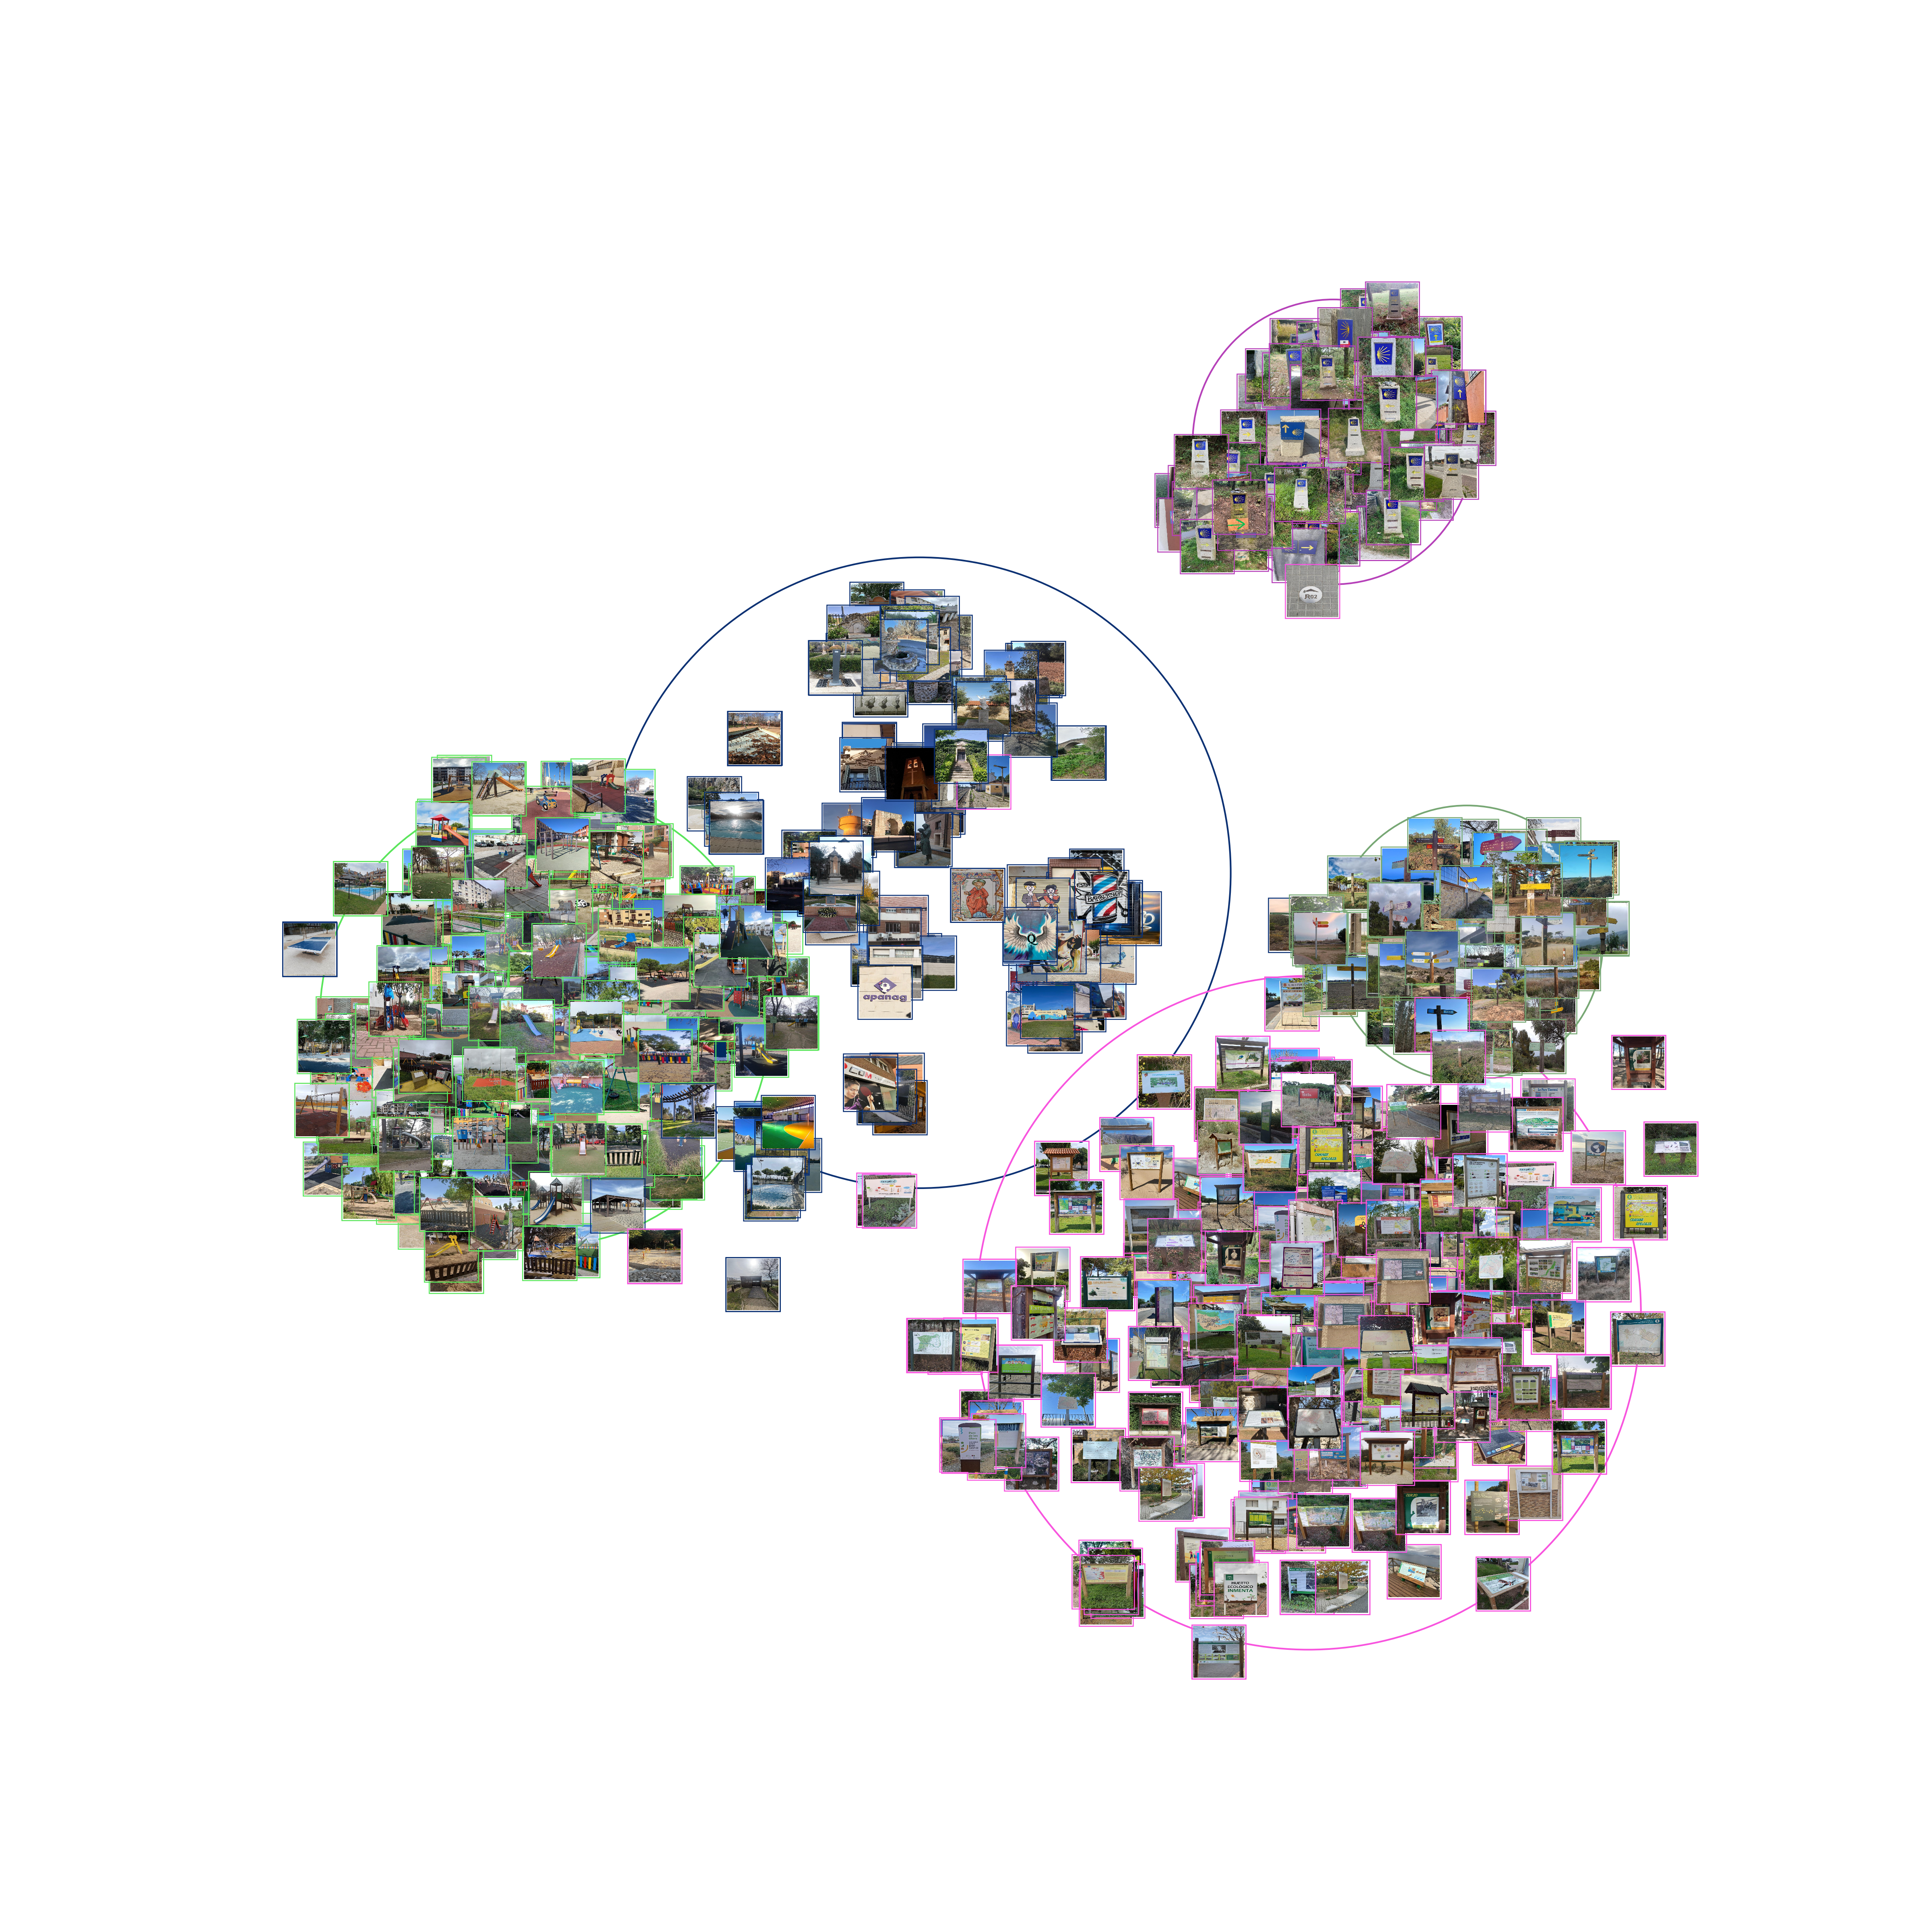
\includegraphics[width = \textwidth]{images_clusters}
					\caption{Imágenes y clusters}
					\label{fig:embeddings_visuales}
				\end{figure} 
				
				En esta situación es mucho más fácil visualizar el resultado obtenido. Se puede observar cómo el transformer ha colocado próximas entre sí las imágenes de cada una de las cuatro clases originales. También ha sido capaz de colocar próximas entre sí a las imágenes que pertenecen a la clase resto, viendo cómo aparecen juntos cada uno de los tipos de objetos que conforman dicha clase, murales, piscinas y fuentes, monumentos, recintos deportivos, esculturas religiosas, etc. Además, hay casos en los que ha ubicado alguna imagen entre varios clusters bien diferenciados, como es el caso de un cartel que aparece entre el cluster de los carteles, el de los parques, y el de otros, en concreto cerca de los elementos deportivos. Pero esto no resulta ser desafortunado, pues al hacer zoom sobre dicha imagen se observa un cartel indicando las normas de un parque con máquinas deportivas. Finalmente, se observa que mediante los colores de los bordes, el algoritmo de clasificación no supervisada ha sido capaz de juntar en el mismo cluster imágenes similares. 
				
			\subsection{Evaluación de la clasificación}
			
				Una vez calculadas las clases o clusters de cada imagen con los dos algoritmos propuestos, se añaden como columnas al dataframe con motivo de agilizar el trabajo de evaluar la calidad de las clasificaciones de embeddings. La \Cref{tab:df_clusters} muestra un extracto. A la hora de realizar la evaluación de la clasificación de los embeddings pueden darse dos situaciones, conocer o no las clases reales. En este caso aprovechando que se conocen las reales, se han abordado ambas situaciones.
			
				\begin{table}[!h]
					\tiny
					\centering
					\texttt{\begin{tabular}{lllrrr}
\toprule
 & imagen & embedding & clase\_original & cluster\_kmeans & cluster\_ac \\
\midrule
10 & camino\_santiago\_13.jpeg & [-0.02232462  0.05146378 -0.03216566 ...  0.00111553  0.01103749
 -0.01471165] & 0 & 2 & 2 \\
447 & marcador\_4.jpeg & [ 0.01137386  0.04624871 -0.0066354  ... -0.01498985  0.02460321
 -0.01014824] & 2 & 0 & 4 \\
821 & resto\_4.jpeg & [-0.02202036  0.06839106 -0.00444437 ... -0.01725521  0.01158767
 -0.05511022] & 4 & 4 & 0 \\
783 & resto\_132.jpg & [ 0.00072823  0.00100317 -0.01555067 ... -0.04994827 -0.04368659
  0.01219591] & 4 & 4 & 0 \\
211 & cartel\_195.jpeg & [0.02073547 0.03421853 0.00191044 ... 0.01309193 0.00961536 0.01201134] & 1 & 3 & 1 \\
\bottomrule
\end{tabular}
}
					\caption{Dataframe con clusters calculados}
					\label{tab:df_clusters}
				\end{table}
				
				\subsubsection{Índice rand ajustado}
				
					En el caso en el que se conocen las clases reales, una de las métricas más populares es el índice rand ajustado o ARI \cite{ari}. Se supone que se dispone de dos particiones del dataset original, $\mathcal{C} = \{C_1, C_2, \ldots, C_r\}$ y $\mathcal{D} = \{D_1, D_2, \ldots, D_s\}$, donde una de ellas es la generada por el algoritmo, y la otra es la original. Con ayuda de cada uno de estos conjuntos se construye la llamada matriz de contingencia, donde la entrada $n_{ij}$ representa el valor de $|C_i \cap D_j|$. En la \Cref{fig:matrices_contingencia} se observan las matrices de contingencia para los clusters generados por los dos algoritmos elegidos. 
					
					\begin{figure}[!h]
						\centering
						\includegraphics[width = \textwidth]{matrices_contingencia}
						\caption{Matrices de contingencia}
						\label{fig:matrices_contingencia}
					\end{figure} 
					
					Estas matrices ayudan a dar una idea de la correspondencia entre los clusters originales y los calculados, observando los elementos que destacan por filas o columnas. Son el primer paso para calcular el ARI, pues sería erróneo pensar que se trata de una clasificación incorrecta el asignar una imagen al cluster $i$, cuando originalmente tenía asignado el cluster $j$, pues puede que sean clusters similares o incluso el mismo, pero que el algoritmo los haya nombrado de diferente manera. Para solucionar este problema, lo que se hace es trabajar con todas las posibles parejas del dataset, y comprobar si pertenecen a las mismas parejas de clusters en ambas particiones, dando lugar a los siguientes cuatro casos. 
					
					\begin{itemize}
						\item $(u \in C_p \,\land\, v \in C_p) \,\land\, (u \in D_q \,\land\, v \in D_q)$
						\item  $(u \in C_p \,\land\, v \in C_p) \,\land\, (u \in D_q \,\land\, v \not\in D_q)$
						\item  $(u \in C_p \,\land\, v \not\in C_p) \,\land\, (u \in D_q \,\land\, v \in D_q)$
						\item  $(u \in C_p \,\land\, v \not\in C_p) \,\land\, (u \in D_q \,\land\, v \not\in D_q)$
					\end{itemize}
					
					A partir de estos casos obtenidos de las matrices de contingencia, se construyen las matrices de confusión que se observan en la \Cref{fig:matrices_confusion_transf}, y que representan la misma idea que en la \Cref{subsub:matriz_confusion}. Se desea que el valor en los elementos de la diagonal principal sea máximo, pues representa el número $A$ de acuerdos; y que sean mínimos el resto, pues representan el valor de desacuerdos $D$. 
					
					\begin{figure}[!h]
						\centering
						\includegraphics[width = \textwidth]{matrices_confusion_transf}
						\caption{Matrices de confusión}
						\label{fig:matrices_confusion_transf}
					\end{figure} 
					
					En este punto se puede calcular el índice rand $\mathcal{R}_I$, que sería el equivalente a la precisión $\mathcal{P}$ presentada en la \Cref{subsub:f1}, pues se calcula como la tasa de acuerdos. En la siguiente ecuación se muestra su cálculo en base a la matriz de contingencia, donde $n_{i\cdot}$ representa la suma de las columnas de la fila $i$, y $n_{\cdot j}$ la suma de las filas de la columna $j$. 
					
					$$
					\mathcal{R}_I = \frac{A}{A + D} = \frac{\displaystyle\binom{n}{2} + 2\sum_{i = 1}^r\sum_{j = 1}^s \binom{n_{ij}}{2} - \sum_{i = 1}^r \binom{n_{i\cdot}}{2} - \sum_{j = 1}^s \binom{n_{\cdot j}}{2}}{\displaystyle\binom{n}{2}}
					$$
					
					Una vez conocido el valor del índice rand, es inmedianto calcular su versión ajustada. Su misión es evitar un valor adecuado por particiones al azar, pues un valor alto de $\mathcal{R}_I$ no necesariamente implica una buena calidad de clustering. Se podría por ejemplo, de manera aleatoria separar el dataset en dos clusters dos veces. Si el número de elementos del dataset es elevado, no sería raro observar que bastantes elementos aparecen en los mismos clusters en ambas particiones, lo que según el $\mathcal{R}_I$ indicaría un buen clustering cuando probablemente no sea así. Se calcula de la siguiente manera. 
					
					$$
					\mathcal{R}_{A_I} = \frac{\mathcal{R}_{I} - E[\mathcal{R}_I]}{\max\{\mathcal{R}_I\} - E[\mathcal{R}_I]} = \frac{\displaystyle\sum_{i = 1}^r\sum_{j = 1}^s\binom{n_{ij}}{2} - \binom{n}{2}^{-1}\sum_{i = 1}^r\binom{n_{i\cdot}}{2}\sum_{j = 1}^s\binom{n_{\cdot j}}{2}}{\displaystyle\frac{1}{2}\left(\sum_{i = 1}^r \binom{n_{i\cdot}}{2} + \sum_{j = 1}^s \binom{n_{\cdot j}}{2}\right) - \binom{n}{2}^{-1}\sum_{i = 1}^r\binom{n_{i\cdot}}{2}\sum_{j = 1}^s\binom{n_{\cdot j}}{2}}
					$$
					
					Valores próximos a 1 indican un buen clustering, cercanos a 0 similar a hacerlo de manera aleatoria, y cercanos a $-1$ (en general menor que cero) peor que de manera aleatoria. Para la clasificación realizada con $k-$means se obtiene un ARI de $0.943$, y con CJA $0.952$. Ambos resultados son muy adecuados. 
					
				\subsubsection{Homogeneidad, completitud, y $V-$measure}
				
					De manera similar que la $F_1-$score relacionaba la precisión y la sensibilidad en el contexto de modelos de clasificación, en el caso de algoritmos de clustering en los que se conocen las clases reales es popular utilizar la $V-$measure, que indica cómo de bueno es el clustering realizado en función de la homogeneidad y completitud de los clusters. Dichos cálculos se basan en la entropía, entropía condicionada y entropía conjunta. 
					
					$$
					\begin{gathered}
						H(\mathscr{C}) = \sum_{i = 1}^{|\mathcal{C}|}P(\mathscr{C}_i)\log_2(P(\mathscr{C}_i))\\
						\begin{aligned}
							H(\mathscr{C} | \mathscr{D}) &= -\sum_{i = 1}^{|\mathcal{C}|}\sum_{j = 1}^{|\mathcal{D}|} P(\mathscr{C}_i \cap \mathscr{D}_j) \log_2 (P(\mathscr{C}_i | \mathscr{D}_j)) &
							H(\mathscr{C}, \mathscr{D}) &= -\sum_{i = 1}^{|\mathcal{C}|}\sum_{j = 1}^{|\mathcal{D}|} P(\mathscr{C}_i \cap \mathscr{D}_j) \log_2 (P(\mathscr{C}_i \cap \mathscr{D}_j))
						\end{aligned}
					\end{gathered}
					$$
					
					En las ecuaciones anteriores \cite{entropia}, los términos $\mathscr{C}$ y $\mathscr{D}$ son variables aleatorias discretas que representan los clusters de las particiones $\mathcal{C}$ y $\mathcal{D}$ a los que pertenece un determiando elemento, y abreviando, $P(\mathscr{C}_i) = P(\mathscr{C} = C_i)$. El concepto de homogeneidad $h$ hace referencia a que cada cluster contenga únicamente elementos de una misma clase; mientras que el de completitud $c$, que todos los miembros de una clase se asignen al mismo cluster \cite{vmeasure}. 
					
					$$
					\begin{aligned}
						h &= \begin{cases}
							1 & \text{si}\, H(\mathscr{C}, \mathscr{D}) = 0\\
							1 - \frac{H(\mathscr{C}|\mathscr{D})}{H(\mathscr{C})} & \text{si}\, H(\mathscr{C}, \mathscr{D}) \neq 0\\
						\end{cases} & 
						c &= \begin{cases}
							1 & \text{si}\, H(\mathscr{D}, \mathscr{C}) = 0\\
							1 - \frac{H(\mathscr{D}|\mathscr{C})}{H(\mathscr{D})} & \text{si}\, H(\mathscr{D}, \mathscr{C}) \neq 0\\
						\end{cases}
					\end{aligned}
					$$
					
					Para los algoritmos de clustering presentados, se obtienen unos valores $(h, c, V)$ adecuados. En el caso de $k-$means se obtiene $(0.923, 0.924, 0.924)$, y para CJA $(0.938, 0.937, 0.937)$. La $V-$measure se calcula de la siguiente manera. 
					
					$$
					V = \frac{2hc}{h + c}
					$$
					
					No es recomendable utilizar esta métrica de manera exclusiva en casos con pocas observaciones (menos de 1000) o un número elevado de clusters (más de 10). En dichos casos es recomendable respaldarla con otras como el ARI. En este caso, se ve como ambas indican un buen clustering.
					
				\subsubsection{Coeficiente de la silueta}
				
					 Otra métrica popular para medir la calidad de un clustering es el coeficiente de la silueta \cite{formulas_silhouette}. Esta no necesita conocer las clases reales, pues mide cómo de parecido es un elemento $\textbf{x}_i$ a los de su cluster, es decir, cómo de compactos son los clusters; y además mide la diferenciación entre clusters, es decir, cómo de separados están. 
					 
					 $$
					 \begin{gathered}
					 	a_i = \frac{1}{|C_l| - 1}\sum_{\substack{\textbf{x}_j\in C_l\\ i\neq j}}\|\textbf{x}_i - \textbf{x}_j\|\\
					 	b_i = \min_{m \neq l}\left\lbrace\frac{1}{|C_m|}\sum_{\textbf{x}_j\in C_m}\|\textbf{x}_i - \textbf{x}_j\|\right\rbrace\\
					 	\mathcal{S} = \frac{1}{n}\sum_{i = 1}^{n}\frac{b_i - a_i}{\text{máx}\{a_i, b_i\}}
					 \end{gathered}
					 $$
					 
					 El cómo de compactos son los clusters lo miden los $a_i$, mientras que la separación entre clusters lo miden los $b_i$. El valor de $\mathcal{S}$ varía entre $-1$ y 1, indicando los valores cercanos a 1 un clustering perfecto (puntos parecidos entre sí en un mismo cluster, y clusters separados), valores cercanos a $-1$ un mal clustering (parecería más razonable asignar algunos puntos a otros clusters), y valores cercanos a cero indican que no estaría claro a qué cluster deberían asignarse algunos puntos al no estar bien separados los clusters \cite{interpretacion_silhouette}. En la \Cref{fig:silhouette_kmeans} se muestra el cálculo del coeficiente de la silueta para el clustering realizado con $k-$means. Se obtiene un valor próximo a cero, indicando que el clustering no es bueno en cuanto a separación de los clusters. \\
					 
					 \begin{figure}[!h]
					 	\centering
					 	\includegraphics[scale = .7]{silhouette_kmeans}
					 	\caption{Coeficiente de la silueta para $k-$means}
					 	\label{fig:silhouette_kmeans}
					 \end{figure} 
				
	\chapter{Conclusiones y trabajo futuro}

	En este trabajo se había planteado como objetivo general el estudio de diferentes técnicas de \gls{nlp}, visión, e inteligencia artificial, con el fin de investigar la posibilidad de automatizar un proceso de valoración de puntos de interés en el mundo real. Esto implicaba tareas con objetivos específicos, como el reconocimiento de objetos en imágenes, y de textos asociados, surgiendo la necesidad de investigar diferentes aproximaciones para resolver estos tipos de problemas, y encontrar la más adecuada. \\
	
	La primera tarea abordada fue la clasificación de imágenes en un conjunto cerrado de clases. Para ello, se decidió utilizar una de las herramientas más populares en problemas de visión artificial que implican tareas como la clasificación o detección de objetos: las redes neuronales convolucionales. Inicialmente, se intentó realizar un entrenamiento desde cero de una \gls{cnn}, lo que resultó en un claro caso de sobreajuste, pues los valores de la función de pérdida sobre el conjunto de validación se disparaban, mientras que los de la función de pérdida sobre el conjunto de entrenamiento tendían a cero. De aquí se obtuvo la conclusión de que se disponía de un número muy reducido de datos de entrenamiento para la cantidad de parámetros a optimizar. A pesar de aplicar técnicas como el aumento de datos, variando parámetros de la imagen como la rotación o el zoom, tampoco se obtuvieron resultados positivos debidos a la insuficiencia datos y persistir el problema del sobreajuste. \\
	
	Ante esta situación, se decidió aplicar la técnica conocida como transfer learning, basada en tomar parámetros de un modelo ya entrenado para un propósito general, de manera que durante el entrenamiento, el resto de parámetros se centren en la tarea específica. En concreto, se tomaron las capas convolucionales del modelo MobileNet de Google, para después añadir capas densas que lograran la clasificación. Gracias a esta técnica, se consiguió eliminar el sobreajuste y clasificar las imágenes en cuatro clases distintas de manera exitosa, obteniendo métricas como un $F_1-$score de $0.97$ o un AuC de $0.99$ sobre un conjunto de imágenes no vistas anteriormente por el modelo. \\
	
	Habiendo conseguido clasificar las imágenes en las cuatro clases originales, se presentó la problemática de poder detectar si una imagen no pertenecía a ninguna de estas. Para ello se plantearon dos soluciones basadas en la anterior. La primera de ellas consistía en añadir una nueva clase a la arquitectura, mientras que la segunda estaba formada por dos \gls{cnn}: una de ellas era capaz de distinguir si una imagen pertenecía a alguna de las clases originales o no, mientras que la otra era capaz de distinguir entre las clases originales. Con el cálculo de probabilidades condicionadas era posible calcular a cuál de las cinco clases (las cuatro originales y una de desconocidos) pertenecía la imagen. Con ambas arquitecturas se obtuvieron resultados muy similares, por lo que se concluyó que era preferible utilizar la primera de ellas, siendo menor el tiempo de cálculo de las predicciones al ser más simple. \\
	
	En este punto se había demostrado que era posible lograr la clasificación de imágenes de un conjunto abierto o cerrado de clases mediante redes convolucionales, pero se presentaban una serie de problemáticas. Si en el futuro se deseaba añadir nuevas clases a las originales, se necesitaba modificar el conjunto de datos, la arquitectura del modelo y reentrenarlo. Además, con la aproximación de \gls{cnn} no se había resulto el problema de trabajar con textos asociados a las imágenes. Tras varias investigaciones surge la idea de trabajar con un tipo de modelos que están a la orden del día, los transformers, específicamente los multimodales, que combinándolos con técnicas de clasificación no supervisada podían solucionar los problemas planteados. \\
	
	Con motivo de añadir un componente de cloud al trabajo, se decidió utilizar un transformer multimodal que es parte de Vertex (\gls{gcp}). Con ayuda de este, se generaron los embeddings de cada imagen, para posteriormente utilizar un algoritmo de clasificación no supervisada como $k-$means o \gls{cja}. Aprovechando que se conocían las clases originales, se utilizaron algunas métricas que proporcionaron valores adecuados, como un ARI de $0.95$ o una $V-$measure de $0.95$. Mediante métricas como el coeficiente de silueta, no se obtuvieron valores óptimos en cuanto a la separación entre clusters, pero las anteriores verificaban la corrección del procedimiento. Gracias a este método, no hacía falta modificar el modelo en caso de desear variar el número de clases, tan solo se debía volver a lanzar el clustering. Además, tampoco era necesario conocer el número de clases, pues mediante el método del codo se podía calcular el óptimo. \\
	
	Con esta arquitectura compuesta por un transformer multimodal y un algoritmo de clasificación no supervisada, se concluyó que era mucho más flexible a cambios futuros en comparación a una basada en \gls{cnn}. Además, permitía resolver el problema de trabajar con textos asociados a las imágenes. La multimodalidad del transformer, permitía generar embeddings de textos en un mismo espacio que los de las imágenes, posibilitando la búsqueda de imágenes mediante descripciones y la selección del texto que mejor describía una imagen. En general, con ayuda del transformer se consiguió extraer de las imágenes detalles más precisos, textos, e incluso agruparlas por conceptos más abstractos. \\
	
	En cuanto a la clasificación de imágenes, se puede afirmar que, independientemente de las tareas relacionadas con texto u otras modalidades de información, la arquitectura formada por un transformer codificador y un algoritmo de clasificación no supervisada es preferible a una basada en \gls{cnn}. Esta combinación ofrece resultados más precisos y es más flexible ante cambios futuros en el dominio del problema, sin la necesidad de reservar datos de entrenamiento. Para finalizar, se propone como trabajo futuro la automatización de las dos tareas con las que se completaría la automatización del proceso de valoración, pues lo relativo a detección de objetos y textos se ha logrado durante este trabajo. \\
	
	La primera de ellas sería detectar los elementos duplicados, es decir, imágenes del mismo objeto en el mismo lugar con diferentes perspectivas. La segunda de ellas sería la verificación de la ubicación proporcionada, por ejemplo  con ayuda de Street View, verificar si el objeto aparece, si el entorno es similar, etc. Para abordar la primera de ellas, se sugiere comenzar utilizando una técnica similar a la empleada para la búsqueda semántica o selección de descripciones. Se puede calcular el coseno del ángulo formado por el embedding de la imagen propuesta y el de cada una de las candidatas a duplicados, tratando de observar los valores de estos. Para el caso de la \Cref{fig:duplicados} se obtienen los valores de $0.89, 0.75, 0.44$, y $0.49$, notándose un valor mayor para la misma imagen tomada desde otra perspectiva, pudiendo ser este el punto de partida de una futura investigación. La segunda de las tareas es bastante más compleja, lo que requeriría el estudio de técnicas más avanzadas de visión artificial, aunque una posible ayuda podría ser recuperar la ubicación de la imagen mediante alguna herramienta como ExifTool, siempre que el usuario no hubiera desactivado los metadatos, para poder calcular la distancia entre las coordenadas. 
	
	\begin{figure}[!h]
		\centering
		\includegraphics[width = .85\textwidth]{duplicados}
		\caption{Imágenes entre las que detectar duplicados}
		\label{fig:duplicados}
	\end{figure}
	
	\addcontentsline{toc}{chapter}{Bibliografía}
	\pagestyle{plain}
	\printbibliography
	
	\appendix
	\chapter{Código y entorno de desarrollo}

	Todo el código desarrollado para llevar a cabo los diferentes experimentos se puede consultar en el siguiente repositorio de GitHub a través del enlace \url{https://github.com/pabloggarc/TFG}. Este es un repositorio que se ha ido utilizando durante el desarrollo del proyecto para llevar un control de versiones del código y la memoria. El contenido se divide en varios directorios. 
	
	\begin{itemize}
		\item \textbf{Anteproyecto}: archivos relacionados con el documento del anteproyecto. 
		\item \textbf{Código}: contiene el código desarrollado para el proyecto. Todos los experimentos mostrados en la memoria suceden en los archivos \texttt{.ipynb}, que son dos notebooks de Python donde aparece el código intercalado con breves comentarios teóricos que han sido extendidos en esta memoria, uno para la parte de redes neuronales convolucionales y otro para la de transformers. Por otro lado, aparecen tres ficheros \texttt{.py}, que son tres scripts utilizados para estructurar los ficheros que forman los datasets. 
		\item \textbf{Diapositivas}: contiene todos los ficheros \LaTeX{} necesarios para generar las diapositivas que se utilizarán para la defensa del proyecto. 
		\item \textbf{Logs}: aparecen en carpetas los diferentes logs generados por TensorFlow durante el entrenamiento de los modelos. Se pueden abrir con TensorBoard para recuperar información y gráficas del entrenamiento. 
		\item \textbf{Memoria}: contiene todos los ficheros \LaTeX{} necesarios para generar esta memoria. 
		\item \textbf{Modelos}: contiene los diferentes modelos entrenados con TensorFlow, listos para poder cargarlos y hacer predicciones. 
	\end{itemize}
	
	Para poder replicar los experimentos, se recomienda replicar el entorno de desarrollo comentado en el \Cref{chapter:practica}. Para ello se debe instalar Ubuntu en su versión 22.04 LTS y LambdaStack mediante el siguiente comando de terminal. 
	\begin{center}
		\begin{BVerbatim}[tabsize = 0]
			wget -nv -O- https://lambdalabs.com/install-lambda-stack.sh | sh -
		\end{BVerbatim}
	\end{center}
	Al instalar ambos elementos se habrá instalado Python, Jupyter, drivers y librerías de NVIDIA, \gls{cuda}, etc. Es importante destacar que para la parte en la que se hace una comparativa entre \gls{cpu} y \gls{gpu}, es necesario disponer de una tarjeta gráfica NVIDIA compatible con \gls{cuda}. Para los entrenamientos, si no se detecta, se harán sobre el procesador automáticamente. \\
	
	Para la parte de transformers, se necesita una cuenta activa en Google Cloud con créditos disponibles, crear un proyecto, e instalar el \gls{cli}. Para ello, basta con ejecutar el siguiente comando de terminal e iniciar sesión. 
	\begin{center}
		\begin{BVerbatim}[tabsize = 0]
			curl https://sdk.cloud.google.com | bash
		\end{BVerbatim}
	\end{center}
	
	% CONTRAPORTADA
	\input{contracubierta}
	
\end{document}